\documentclass{beamer} 
\usetheme{metropolis}
\usepackage{listings}
\usepackage{amsfonts}
\usepackage{dsfont}
\usepackage{amsmath}
\usepackage{bbm}
\usepackage{verbatim}
%\usepackage{tipa}
\usepackage{tikz}
\usetikzlibrary{fit}
\usepackage{color}
\usepackage{booktabs}
\usepackage{tipa}
\usepackage{amssymb}
\usepackage{verbatim}
\usepackage[absolute,overlay]{textpos}
\usepackage{pifont}% http://ctan.org/pkg/pifont
\usepackage{caption}
\usepackage{subcaption}
\newcommand{\cmark}{\ding{51}}%
\newcommand{\xmark}{\ding{55}}%
\usetikzlibrary{bayesnet}
\usetikzlibrary{decorations.markings}
\usetikzlibrary{decorations.pathmorphing}
\tikzset{squiggle/.style={decorate, decoration={snake,amplitude=.4mm}}}
\usepackage{xcolor}
\definecolor{pop1}{HTML}{1F78b4}
\definecolor{pop2}{HTML}{164C13}
\definecolor{pop3}{HTML}{d95F02}
\definecolor{orange}{HTML}{d95F02}
\definecolor{teal}{HTML}{1b9e77}
\newcommand{\pop}[1]{\textcolor{pop1}{#1}}
\newcommand{\popp}[1]{\textcolor{pop2}{#1}}
\newcommand{\tree}[1]{\textcolor{pop3}{#1}}
\newcommand{\orange}[1]{\textcolor{orange}{#1}}
\newcommand{\teal}[1]{\textcolor{teal}{#1}}
\newcommand{\code}[1]{{\footnotesize\texttt{#1}}}
\newcommand{\greenCode}[1]{{\footnotesize\popp{\code{#1}}}}
\newcommand{\blueCode}[1]{{\footnotesize\pop{\code{#1}}}}


\usepackage{pgf}  



\newcommand{\nextForm}[1]{\rotatebox[origin=c]{270}{$_{\curvearrowright}$}$_{#1}$}
 
\usepackage{amsfonts}
\usepackage{tabularx}
%\usepackage{color}
\usepackage{graphicx}
\usepackage{booktabs}
\usepackage{xcolor}
\usepackage{tikz}
\usetikzlibrary{trees}
\usetikzlibrary{fit}
\usetikzlibrary{calc}
\usetikzlibrary{bayesnet}
\usepackage[absolute,overlay]{textpos}
\usepackage{stmaryrd}
\newcommand{\sem}[1]{\llbracket #1\rrbracket}
\newcommand{\tuple}[1]{\ensuremath{\left \langle #1\right \rangle}}
\usepackage{booktabs}
\usepackage{tipa}
\usepackage{amssymb}
\usepackage{verbatim}
\usepackage[absolute,overlay]{textpos}
\usepackage{pifont}% http://ctan.org/pkg/pifont
\newcommand{\cmark}{\ding{51}}%
\newcommand{\xmark}{\ding{55}}%
\usetikzlibrary{bayesnet}
\usetikzlibrary{decorations.markings}

\newcommand\Wider[2][3em]{%
\makebox[\linewidth][c]{%
  \begin{minipage}{\dimexpr\textwidth+#1\relax}
  \raggedright#2
  \end{minipage}%
  }%
}


\usepackage[utf8]{inputenc}

\usepackage{amssymb}% http://ctan.org/pkg/amssymb
\usepackage{pifont}% http://ctan.org/pkg/pifont

\usepackage{fancyvrb}

\usepackage[most]{tcolorbox}
\definecolor{block-gray}{gray}{0.10}
\newtcolorbox{mycode}{colback=block-gray,grow to right by=0mm,grow to left
by=0mm, boxrule=0pt,boxsep=0pt,breakable,fontupper=\color{white}}

%% Program ::=
%%   (if Bool List
%%     (append RecursiveList
%%             RecursiveList
%%             RecursiveList))
%% RecursiveList ::= List
%%          | (recurse List)

            

\usepackage{arydshln}

\newcommand{\Expect}{\mathds{E}} %{{\rm I\kern-.3em E}}
\newcommand{\Probability}{\mathds{P}} %{{\rm I\kern-.3em P}}

\DeclareMathOperator*{\argmax}{arg\,max}
%Information to be included in the title page:
\title{\texttt{DreamCoder}: Growing libraries of concepts with wake-sleep program induction}
\author{Kevin Ellis\\Joint with: Lucas Morales, Mathias Sabl\'e Meyer, Armando Solar-Lezama, Joshua B. Tenenbaum\\Heavy inspiration from: Eyal Dechter}
\institute{MIT} 
\date{October 2018}
  
 
\begin{document}
 
\frame{\titlepage}



\begin{frame}{Human program induction everywhere}
\begin{tikzpicture}
  \node(Lisp) at (0,0) {\includegraphics[width = 5cm]{figures/1975.png}};
  \visible<2->{
    \node(colorless) at (6,0) {\includegraphics[width = 5cm]{figures/colorless.png}};
    \node at ([yshift=-2cm]colorless.south) {\includegraphics[width = 4cm]{figures/child.jpg}};
  }
  \visible<3->{
    \node(aqueduct) at ([yshift=-1cm,xshift=0cm]Lisp.south) {\includegraphics[width = 5cm]{figures/aqueduct.jpg}};
    \node(arch) at ([xshift=1cm,yshift=0cm]aqueduct.south) {\includegraphics[width = 1.5cm]{figures/arch.jpg}};
  }
  \visible<4->{
    \node at ([yshift=-1cm,xshift=-2cm]aqueduct.south) {\includegraphics[width = 2cm]{figures/tapestry.jpg}};
    \node(wiringDiagram) at ([yshift=-1cm,xshift=1.6cm]aqueduct.south) {\includegraphics[width = 5cm]{figures/wiringDiagram.jpg}};
  }
  %% \visible<5->{
  %%   \node at ([xshift=2cm,yshift=1cm]wiringDiagram.east) {\includegraphics[width = 5cm]{tree.jpg}};
  %%   }
  \end{tikzpicture}

\end{frame}

%% \begin{frame}{Engineering the language of thought}
%%  \begin{tikzpicture}
%%     \node () {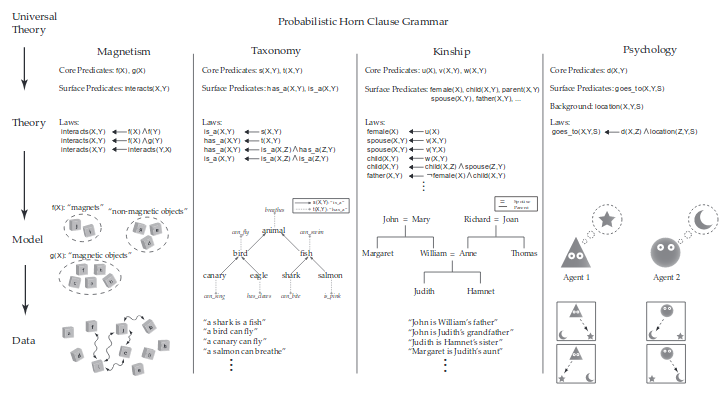
\includegraphics[width = 15.6cm]{theory.png}};
%%     \node at (-5,-4) {  Ullman et al 2012};
%%     \end{tikzpicture}
%% \end{frame}

\begin{frame}{Human program induction everywhere}
  \begin{tikzpicture}
    \node at(0,0) {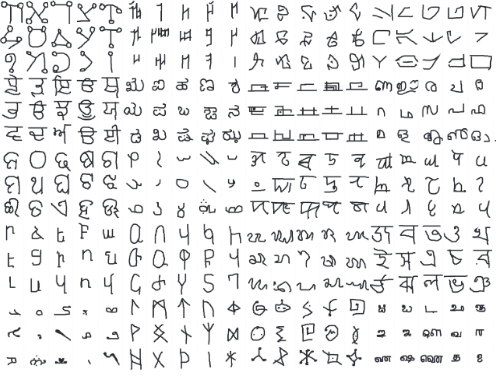
\includegraphics[width = 8cm]{characters.png}};
    \node at(-3,2) {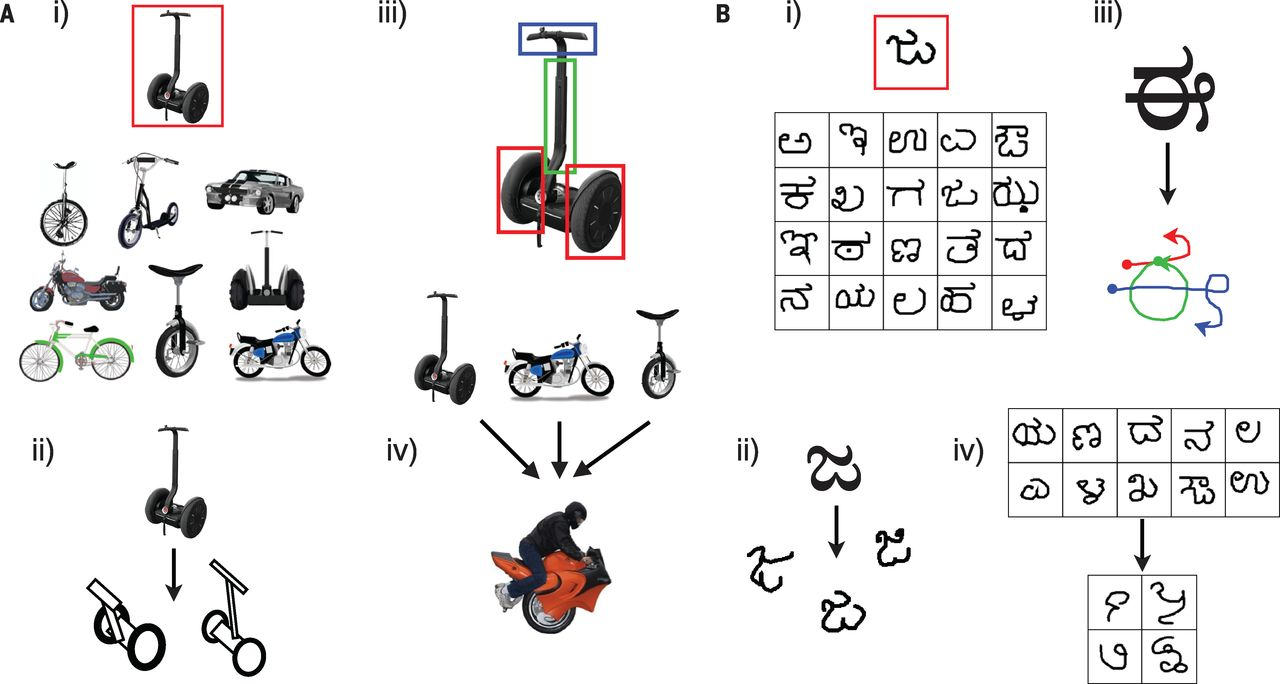
\includegraphics[width = 8cm]{Brendan.jpg}};

    \node at (-5,-4) {  Lake et al 2015};
    \end{tikzpicture}
\end{frame}





\begin{frame}{Growing domain-specific knowledge}
  
  %  \Large
  Goal: acquire domain-specific knowledge needed to induce a class of programs


  
  \vspace{1cm}

  \begin{itemize}
  \item Library of concepts (declarative knowledge; generative model over programs)
    \item Inference strategy (procedural knowledge)
  \end{itemize}
  \only<2>{
  \begin{tikzpicture}
    \node(problem) at (0,0) {
\includegraphics[width = 2cm]{figures/functions/48.png}};
    \node(synthesizer)[draw,align=center] at ([xshift=3cm]problem.east) {Learned \\program inducer};
    \draw[->] (problem.east) -- (synthesizer.west);
    \node(program)[draw, align=center] at ([xshift=3cm]synthesizer.east) {program:\\$f(x) = 0.7x^2+1.2$};
    \draw[->] (synthesizer.east) -- (program.west);
  \end{tikzpicture}
  
    \vspace{0.2cm}Concepts: $x^2$, etc\\Inference strategy: neurosymbolic search for programs}
  \renewcommand\code\texttt
    \only<3>{
  \begin{tikzpicture}
    \node(problem) at (0,0) {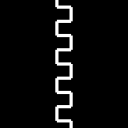
\includegraphics[width = 2cm]{figures/logoTasks/logo43.png}};
    \node(synthesizer)[draw,align=center] at ([xshift=3cm]problem.east) {Learned \\program inducer};
    \draw[->] (problem.east) -- (synthesizer.west);
    \node(program)[draw, align=center] at ([xshift=3cm]synthesizer.east) {program:\\\code{(for (i 4)}\\ \code{ (circle i))}};
    \draw[->] (synthesizer.east) -- (program.west);
  \end{tikzpicture}
  
  \vspace{0.2cm}Concepts: \code{circle}, etc\\Inference strategy: neurosymbolic search for programs
    }
%%     \only<4>{
%% \Wider[4em]{  \begin{tikzpicture}
%%     \node[draw,align=center](problem) at (0,0) {
%%             \begin{tabular}{l}
%%           \code{[7\, 2\, 3]}$\to$\code{[7\, 3]}         \\
%%           \code{[1\, 2\, 3\, 4]}$\to$\code{[3\, 4]} \\
%%           \code{[4\, 3\, 2\, 1]}$\to$\code{[4\, 3]} \\
%%           \end{tabular}
%% };
%%     \node(synthesizer)[draw,align=center] at ([xshift=2.5cm]problem.east) {Learned \\program inducer};
%%     \draw[->] (problem.east) -- (synthesizer.west);
%%     \node(program)[draw, align=center] at ([xshift=2.5cm]synthesizer.east) {program:\\\code{(filter ($\lambda$ (x)}\\\code{ (> x 2)))}};
%%     \draw[->] (synthesizer.east) -- (program.west);
%%   \end{tikzpicture}

%%   \vspace{0.5cm}Concepts: \code{filter}, etc\\Inference strategy: neurosymbolic search for programs
%%     }}
  
\end{frame}

\begin{frame}{DSL: Library of concepts}
\Wider[5.4em]{
  \renewcommand\code\texttt
  \renewcommand\codechar[1]{\texttt{"#1"}}
  \newcommand{\helpSize}{0.25cm}
  \footnotesize\begin{tabular}{cc}
    \toprule
Tasks and     \pop{Programs} & DSL\\
    \midrule
      \begin{tabular}{cc}
        \begin{tabular}{c}
          \code{[7\, 2\, 3]}$\to$\code{[7\, 3]}         \\
          \code{[1\, 2\, 3\, 4]}$\to$\code{[3\, 4]} \\
          \code{[4\, 3\, 2\, 1]}$\to$\code{[4\, 3]} \\
          \pop{\code{$f(\ell) = $}\code{($f_1$ $\ell$ ($\lambda$ (x)}}\\
          \hspace{1.15cm}\pop{\code{(> x 2)))}}       \\
          \\
          \\
          \code{[2\, 7\, 8\, 1]}$\to $\code{8}               \\
          \hspace{0.15cm}\code{[3\, 19\, 14]}$\to $\code{19}                \\
          \pop{\code{$f(\ell) = $}\code{($f_2$ $\ell$)}}
        \end{tabular}
        &
        \hspace{-0.3cm}\begin{tabular}{c}
          \code{[7\, 3]}$\to $\code{False}                              \\
          \hspace{0.3cm}\code{[3]}$\to $\code{False}                    \\
          \hspace{-0.3cm}\code{[9\, 0\, 0]}$\to $\code{True\phantom{e}} \\
          \hspace{0.3cm}\code{[0]}$\to $\code{True\phantom{e}}                        \\
          \hspace{-0.3cm}\code{[0\, 7\, 3]}$\to $\code{True\phantom{e}}                \\
          \pop{\code{$f(\ell) = $}\code{($f_3$ $\ell$ 0)}}
        \end{tabular}
      \end{tabular}
    &
    \begin{tabular}{l}
      \popp{$f_0(\ell,$\code{r}$) \,=\, $\code{(foldr r $\ell$ cons)}}\\
      \hspace{\helpSize}($f_0$: \emph{Append lists }\code{r}\emph{ and  $\ell$})\\
      \popp{$f_1(\ell,$\code{p}$) \,=\, $\code{(foldr $\ell$ nil ($\lambda$ (x a)}}\\
      \hspace{0.5cm}\popp{\code{(if (p x) (cons x a) a)))}}\\
      \hspace{\helpSize}($f_1$: \emph{Higher-order filter function})\\
      %(lambda (fold $0 0 (lambda (lambda (if (gt? $0 $1) $0 $1)))))
      \popp{$f_2(\ell) \,=\, $\code{(foldr $\ell$ 0 ($\lambda$ (x a)}}\\
      \popp{\phantom{$f_2(\ell) \,=\, $}\code{(if (> a x) a x)))}}\\
      \hspace{\helpSize}($f_2$: \emph{Maximum element in list $\ell$})\\
      \popp{$f_3(\ell,$\code{k}$) \,=\, $\code{(foldr $\ell$ (is-nil $\ell$)}}\\
      \phantom{$f_1(\ell,$}
      \popp{\code{($\lambda$ (x a) (if a a (= k x))))}}\\
      \hspace{\helpSize}($f_2$: \emph{Whether $\ell$ contains }\code{k})\\
    \end{tabular}
  \\\bottomrule
  \end{tabular}
}
\end{frame}

\begin{frame}{DreamCoder}
  \begin{itemize}
  \item   \textbf{Wake:} Solve problems by writing programs
  \item \textbf{Sleep:} Improve DSL and neural recognition model:
    \begin{itemize}
    \item \textbf{Sleep-G:} Improve DSL (\textbf{G}enerative model)
      \item \textbf{Sleep-R:} Improve \textbf{R}ecognition model
      \end{itemize}
  \end{itemize}
  Combines ideas from Wake-Sleep \& Exploration-Compression algorithm by Eyal Dechter
\Wider[5.4em]{
  \begin{tikzpicture}
    \node at (6,0) {  \includegraphics[width = 4cm]{figures/sleepingChild.jpg}};
    \visible<2->{
      \node(Lisp) at (-3,0) {\includegraphics[width = 3cm]{figures/Lisp.png}};
      \node[align=center](tower) at ([xshift=1cm]Lisp.east) {
\includegraphics[width = 1cm]{figures/functions/627.png}\hspace{0.05cm}
\includegraphics[width = 1cm]{figures/functions/615.png}\\
        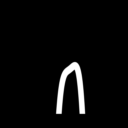
\includegraphics[width = 1cm]{figures/functions/382.png}\hspace{0.05cm}
\includegraphics[width = 1cm]{figures/functions/0.png}%
      };
      \node(logo) at ([xshift=1.5cm]tower.east) {\includegraphics[width =3cm]{figures/9logo.png}}; 
    }
    \end{tikzpicture}}


\end{frame}
\begin{frame}[t]{DSL learning as Bayesian inference}
  %  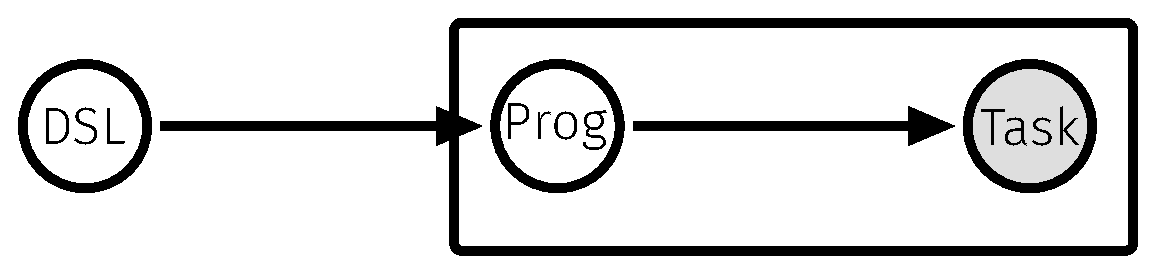
\includegraphics[width = 11cm]{figures/animation/EC.eps}
\centering  \begin{tikzpicture}[scale=1.3,line width=0.5mm]

  \node[latent,scale=1] at (3.5,3) (dx){DSL};
  \node[latent,scale=1] at ([yshift=-1.5cm]dx) (zp){prog};
  \node[obs,scale=1] at ([yshift=-2cm]zp) (xp) {data};
  \node[latent,scale=1] at ([xshift=2cm]zp) (zp1){prog};
  \node[obs,scale=1] at ([xshift=2cm]xp) (xp1) {data};
  \draw [->] (zp1.south) -- (xp1.north);
  \draw [->] (dx.south) -- (zp1.north);
  %\draw [->,red] (xp1.east) to[out = 30,in = -30] node(nn){} (zp1.east);
%  \node at (nn) {\NeuralNetwork{0.5}};
  % HACK : "invisible" arrow to phantom and push to the left and align with next
  % slide
  \draw [->,red,opacity=0.0001] (xp1.east) to[out = 30,in = -30] node(nn){} (zp1.east);
  
  \node[latent,scale=1] at ([xshift=-2cm]zp) (zp1){prog};
  \node[obs,scale=1] at ([xshift=-2cm]xp) (xp1) {data};
  \draw [->] (zp1.south) -- (xp1.north);
  \draw [->] (dx.south) -- (zp1.north);
%  \draw [->,red] (xp1.east) to[out = 30,in = -30] node(nn){} (zp1.east);
%  \node at (nn) {\NeuralNetwork{0.5}};


%  \draw [->,red] (xp.east) to[out = 30,in = -30] node(nn){} (zp.east);
 % \node at (nn) {\NeuralNetwork{0.5}};
  \draw [->] (dx.south) -- (zp.north);
  \draw [->] (zp.south) -- (xp.north);


  %\node[shift={+(0,-1.7)}] at (nn) { $Q$  };

  \end{tikzpicture}
  

\vspace{0.5cm}
  
\textbf{[Dechter et al., 2013]}  [Liang et al, 2010]; [Lake et al, 2015]

\textbf{Dechter et al.}: Exploration-Compression. Inspiration for DreamCoder.

  %% \vfill
  %% Gray: Observed.\\
  %% White: Latent.\\
  %% Boxed (plate): Repeated.\\
  
\end{frame}
\newcommand{\NeuralNetwork}[1]{    \begin{tikzpicture}[x=2.5cm,y=1.25cm,transform canvas={scale=#1,shift={+(-1,2.5)}}]
      \tikzstyle{neuron}=[circle,fill=blue!50,minimum size=20pt]
      \fill[fill=white] (-0.25,-0.5) rectangle (2.25,-4.5);
      \node[rectangle] at (1,1) {};
      \foreach \name / \y in {1,...,4}
          \node[neuron] (I-\name) at (0,-\y) {};
      \foreach \name / \y in {1,...,3}
          \node[neuron] (H-\name) at (1,-\y-0.5) {};
      \foreach \name / \y in {1,...,4}
          \node[neuron] (O-\name) at (2,-\y) {};
      \foreach \source in {1,...,4}
          \foreach \dest in {1,...,3}
              \draw [-latex] (I-\source) -- (H-\dest);
      \foreach \source in {1,...,3}
          \foreach \dest in {1,...,4}
              \draw [-latex] (H-\source) -- (O-\dest);
    \end{tikzpicture}}
\begin{frame}[t]{DSL learning as \alert{amortized} Bayesian inference}
\centering  \begin{tikzpicture}[scale=1.3,line width=0.5mm]

  \node[latent,scale=1] at (3.5,3) (dx){DSL};
  \node[latent,scale=1] at ([yshift=-1.5cm]dx) (zp){prog};
  \node[obs,scale=1] at ([yshift=-2cm]zp) (xp) {data};
  \node[latent,scale=1] at ([xshift=2cm]zp) (zp1){prog};
  \node[obs,scale=1] at ([xshift=2cm]xp) (xp1) {data};
  \draw [->] (zp1.south) -- (xp1.north);
  \draw [->] (dx.south) -- (zp1.north);
  \draw [->,red] (xp1.east) to[out = 30,in = -30] node(nn){} (zp1.east);
%  \node at (nn) {\NeuralNetwork{0.5}};
  
  \node[latent,scale=1] at ([xshift=-2cm]zp) (zp1){prog};
  \node[obs,scale=1] at ([xshift=-2cm]xp) (xp1) {data};
  \draw [->] (zp1.south) -- (xp1.north);
  \draw [->] (dx.south) -- (zp1.north);
  \draw [->,red] (xp1.east) to[out = 30,in = -30] node(nn){} (zp1.east);
%  \node at (nn) {\NeuralNetwork{0.5}};


  \draw [->,red] (xp.east) to[out = 30,in = -30] node(nn){} (zp.east);
  \node at (nn) {\NeuralNetwork{0.25}};
  \draw [->] (dx.south) -- (zp.north);
  \draw [->] (zp.south) -- (xp.north);


  %\node[shift={+(0,-1.7)}] at (nn) { $Q$  };

\end{tikzpicture}



\textbf{New:} amortized inference +\\ better program representation (Lisp) + \\better DSL inference 

\end{frame}
\begin{frame}{Wake --- as in Exploration/Compression Algorithm}
  \only<1>{
    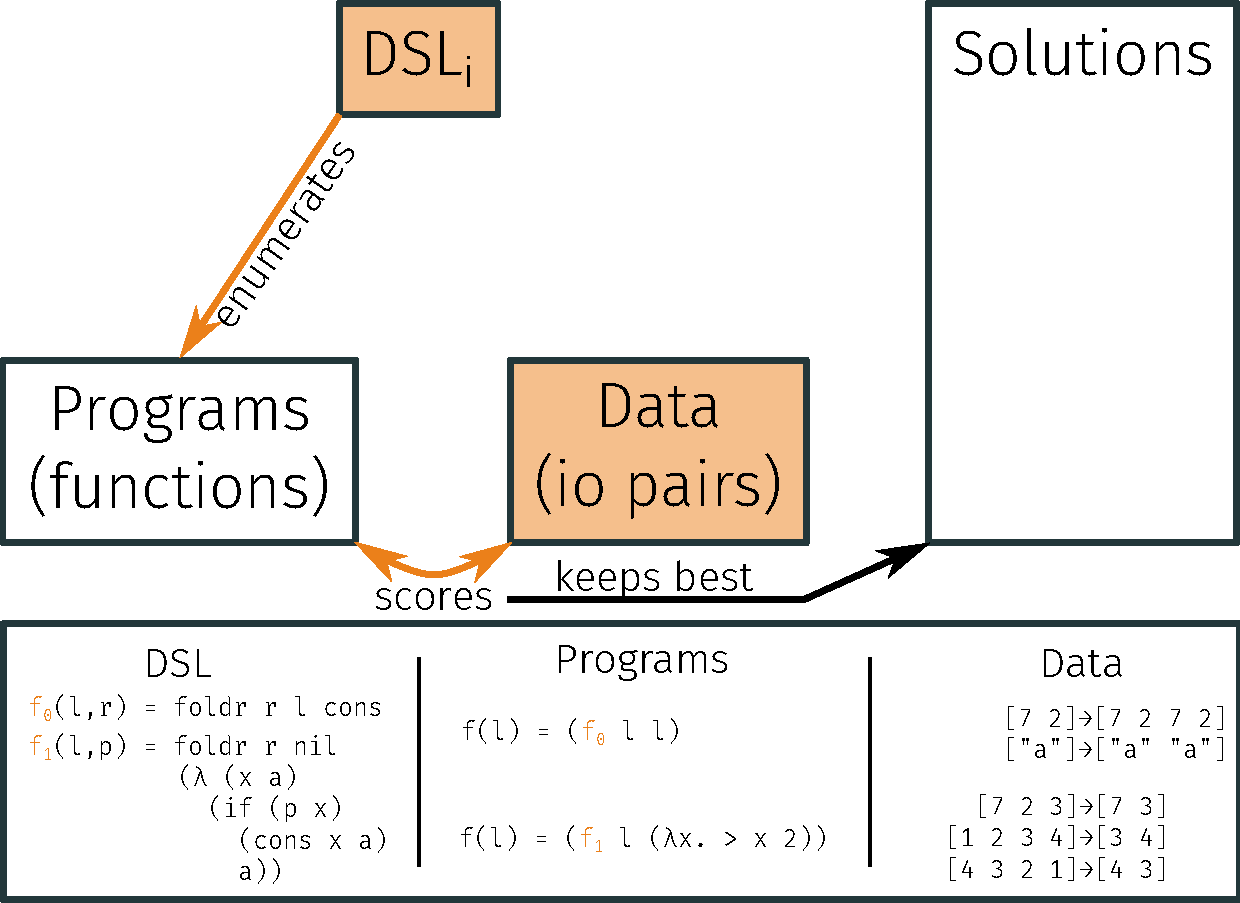
\includegraphics[width=11cm]{figures/teachDC/.inkslides-ec/slide-0.pdf}
  }
  \only<2>{
    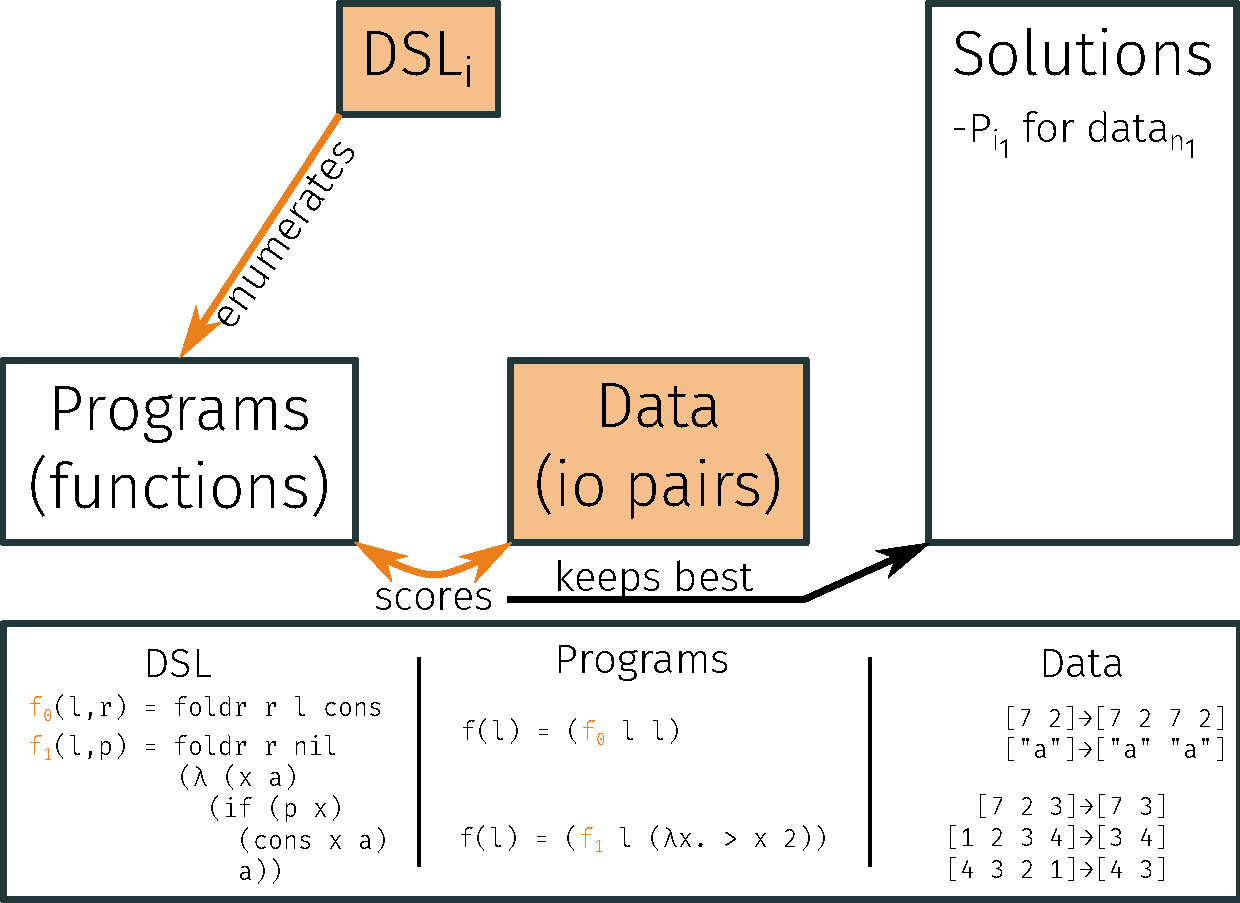
\includegraphics[width=11cm]{figures/teachDC/.inkslides-ec/slide-1.pdf}
  }
  \only<3>{
    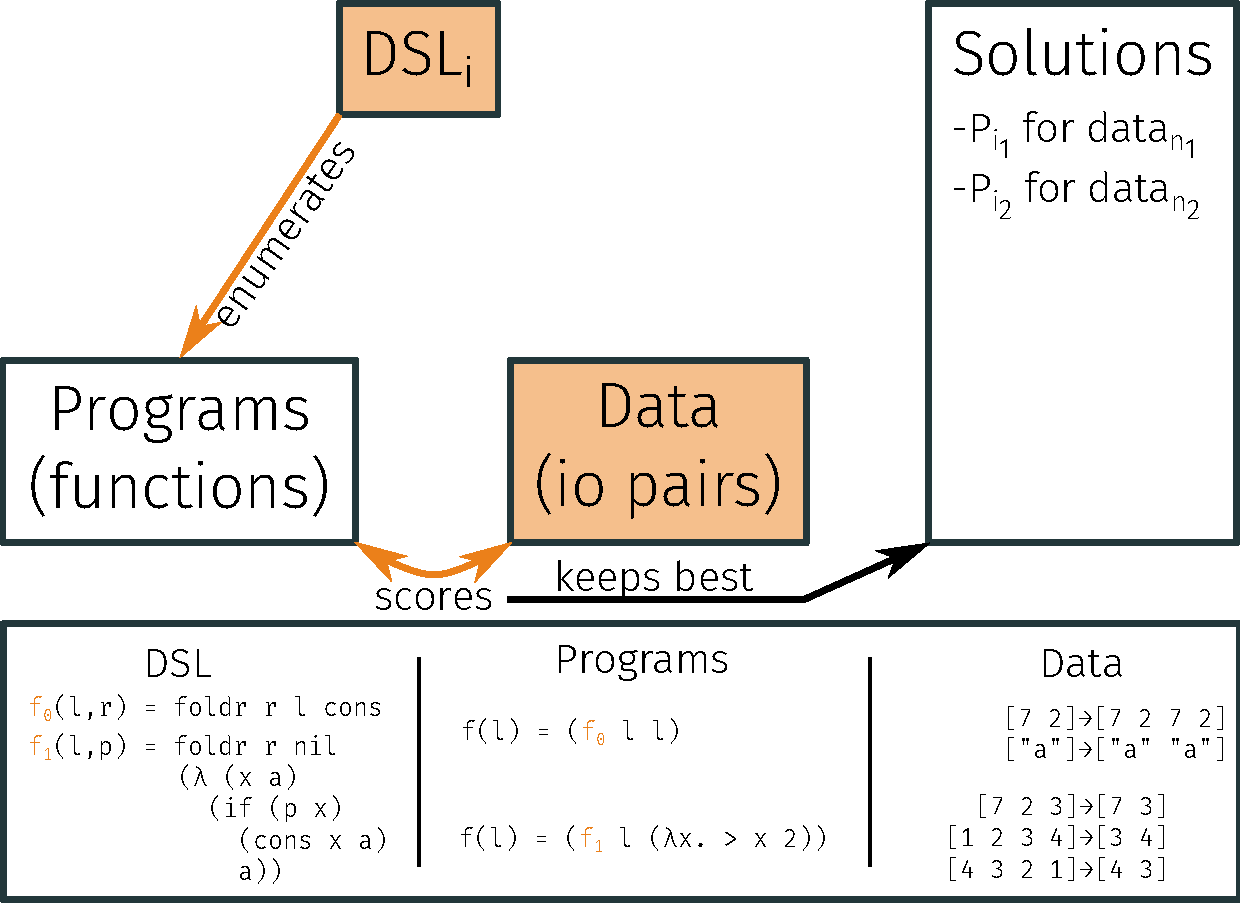
\includegraphics[width=11cm]{figures/teachDC/.inkslides-ec/slide-2.pdf}
  }
  \only<4>{
    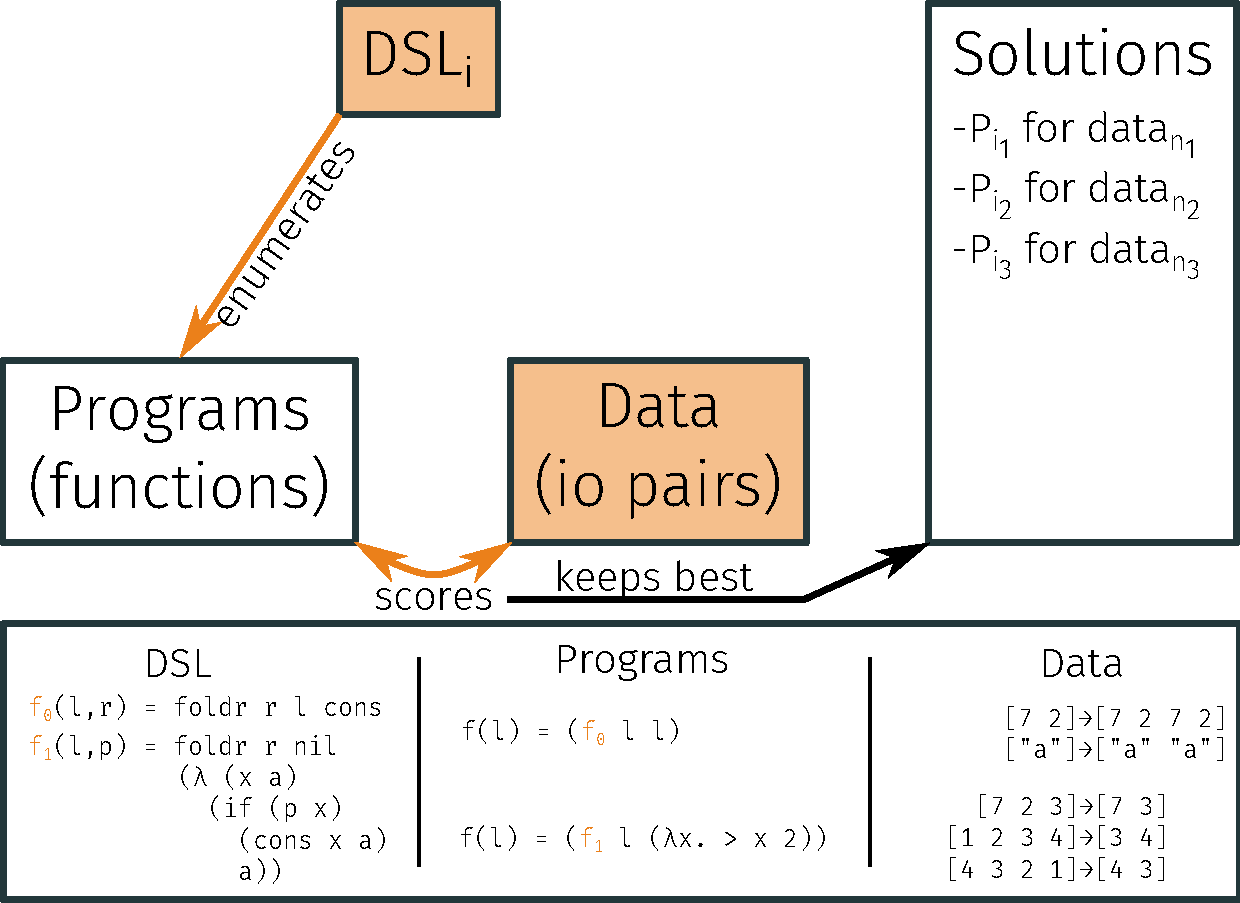
\includegraphics[width=11cm]{figures/teachDC/.inkslides-ec/slide-3.pdf}
  }
  \only<5>{
    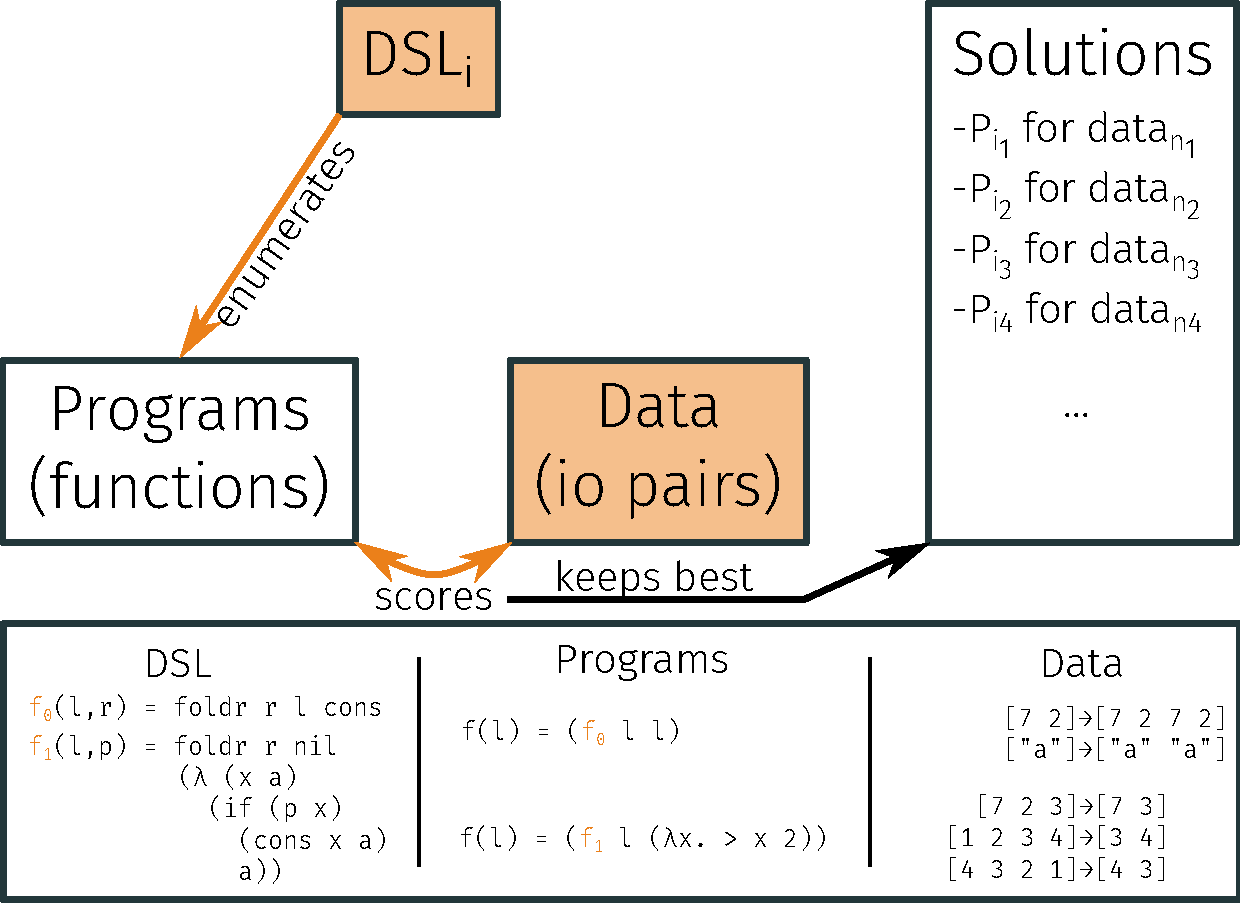
\includegraphics[width=11cm]{figures/teachDC/.inkslides-ec/slide-4.pdf}
  }

\end{frame}

\begin{frame}{DreamCoder --- Wake}
  \only<1>{
    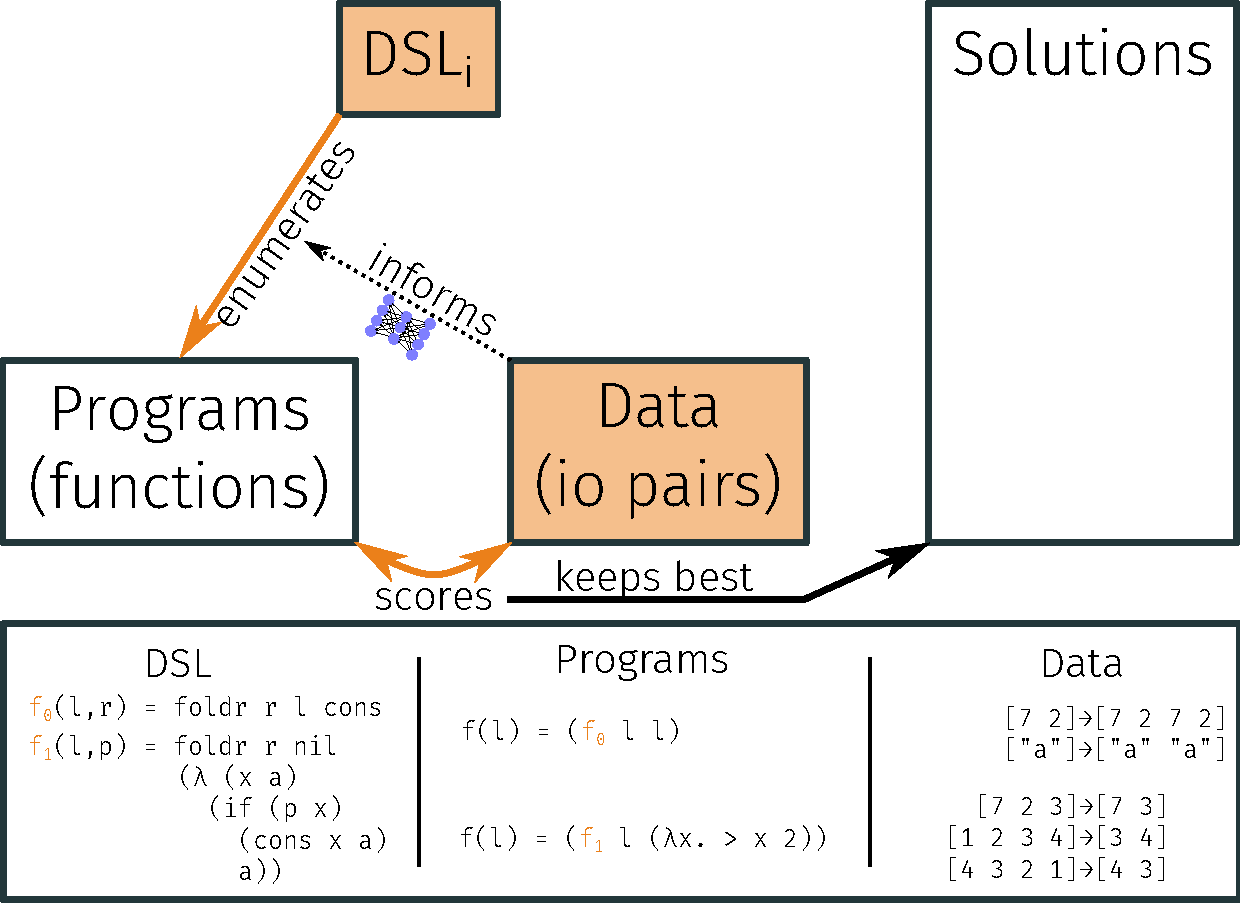
\includegraphics[width=11cm]{figures/teachDC/.inkslides-dc/slide-0.pdf}
  }
  \only<2>{
    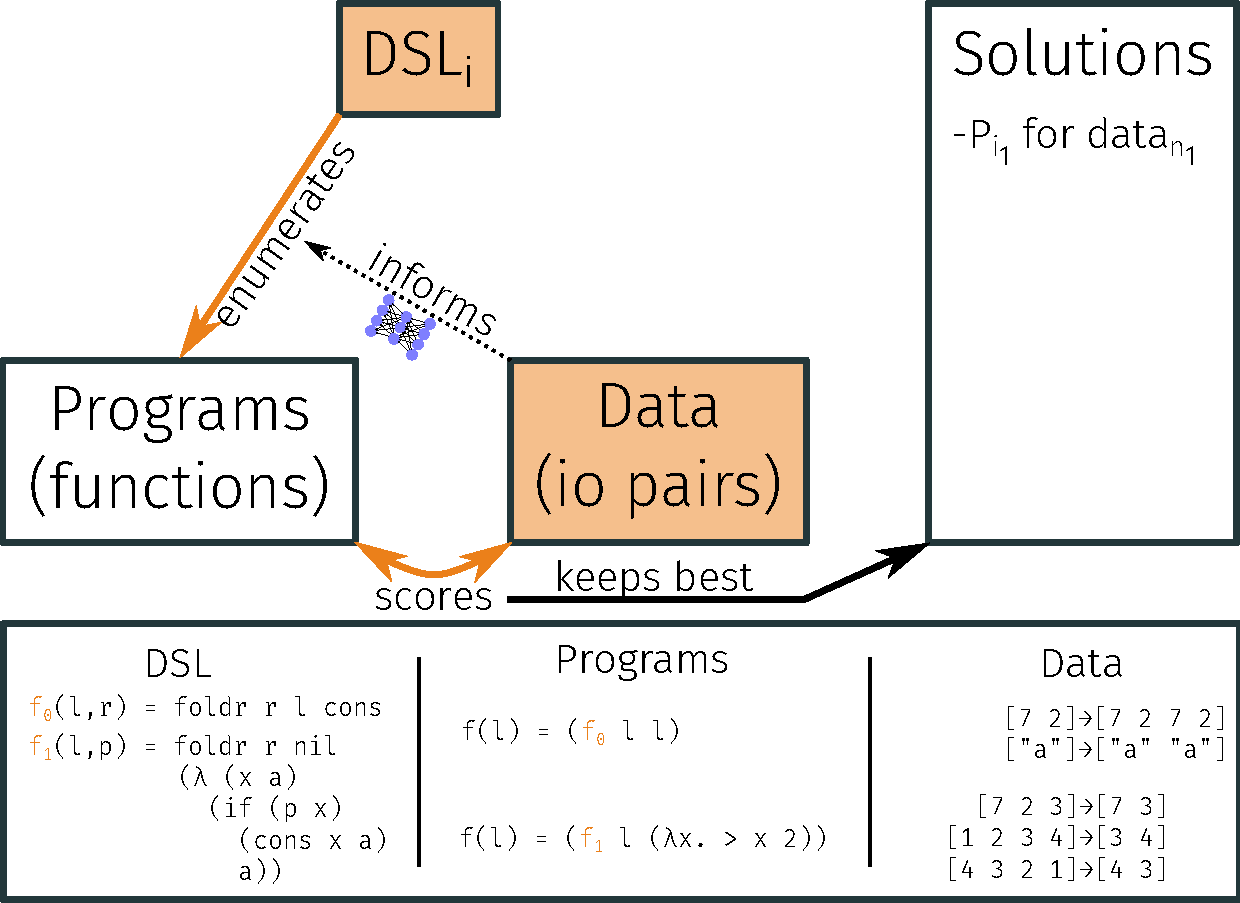
\includegraphics[width=11cm]{figures/teachDC/.inkslides-dc/slide-1.pdf}
  }
  \only<3>{
    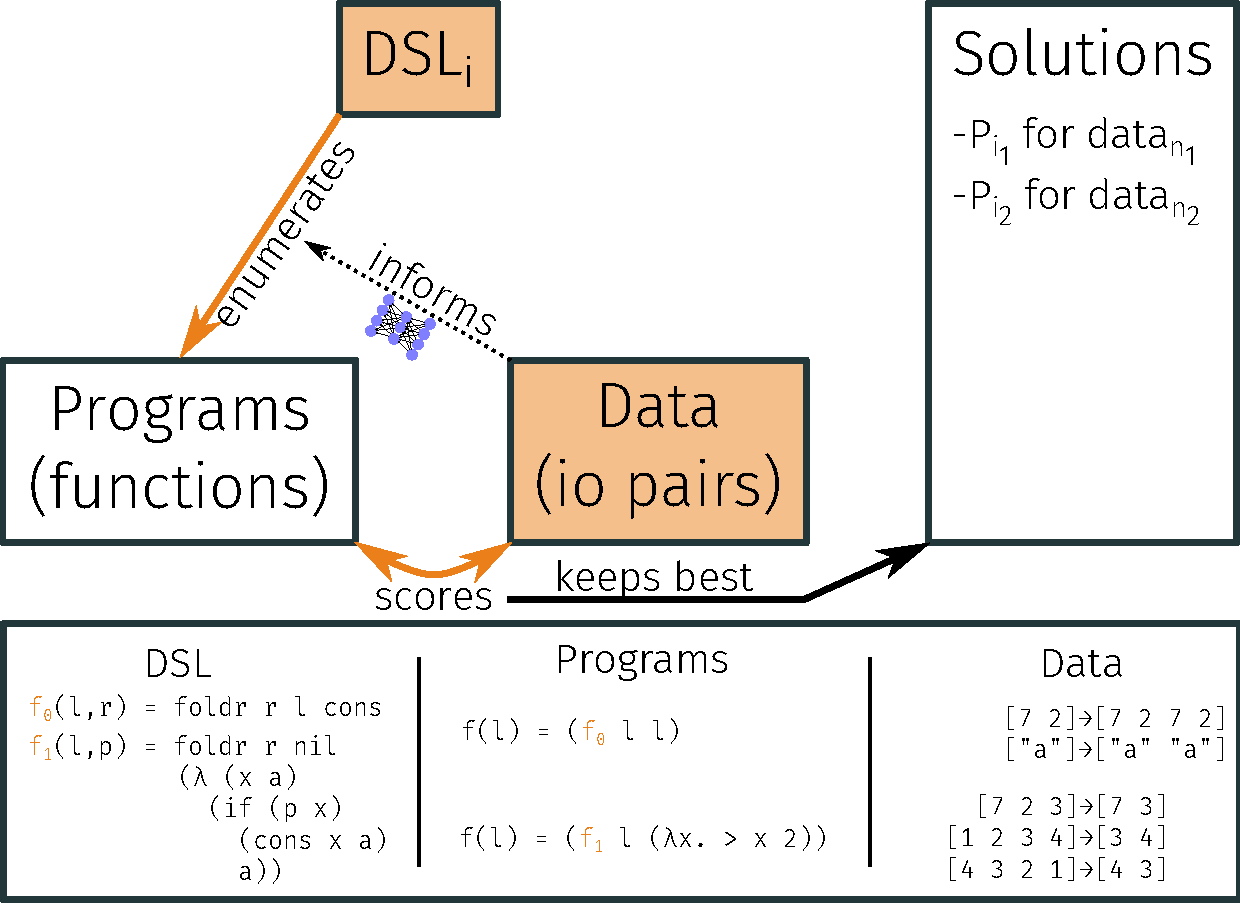
\includegraphics[width=11cm]{figures/teachDC/.inkslides-dc/slide-2.pdf}
  }
  \only<4>{
    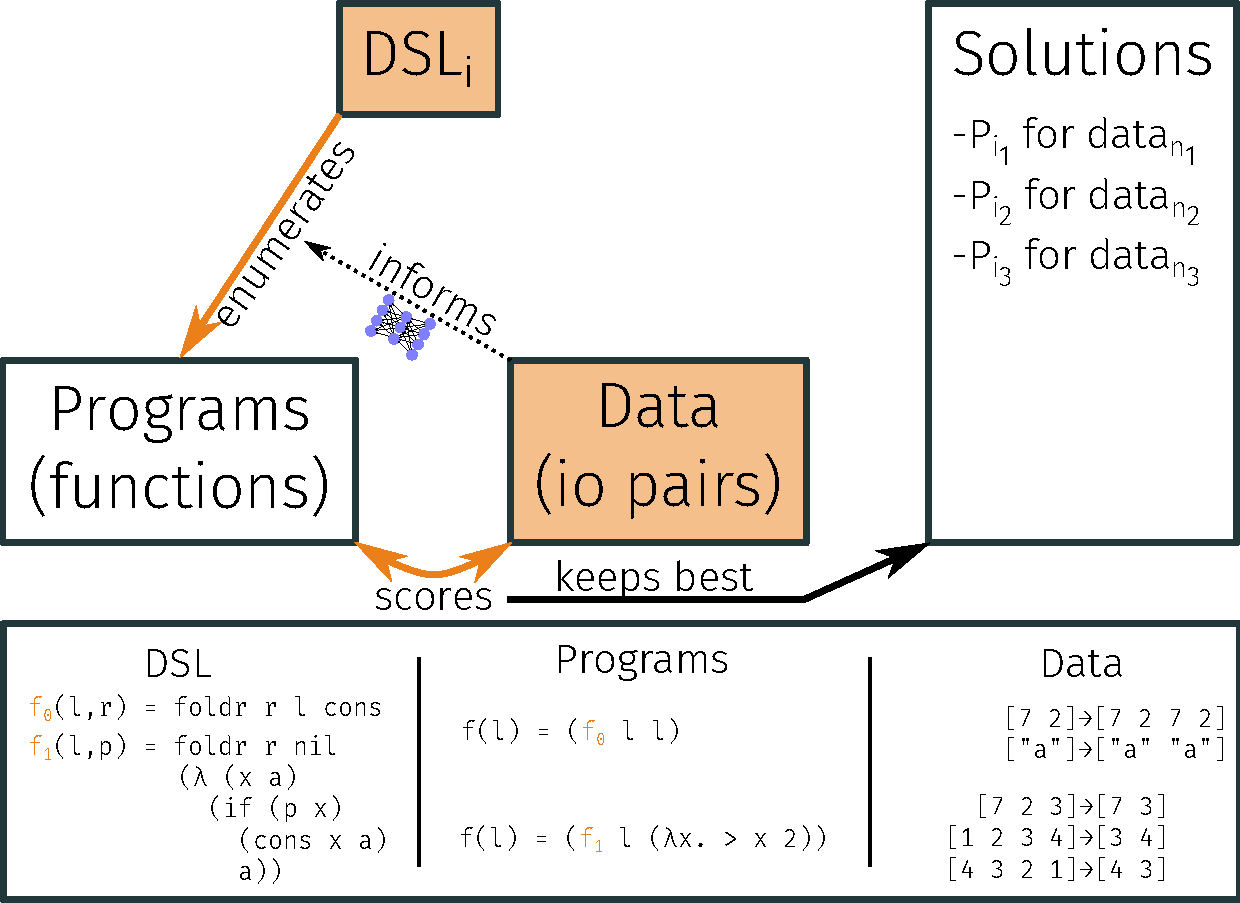
\includegraphics[width=11cm]{figures/teachDC/.inkslides-dc/slide-3.pdf}
  }
  \only<5>{
    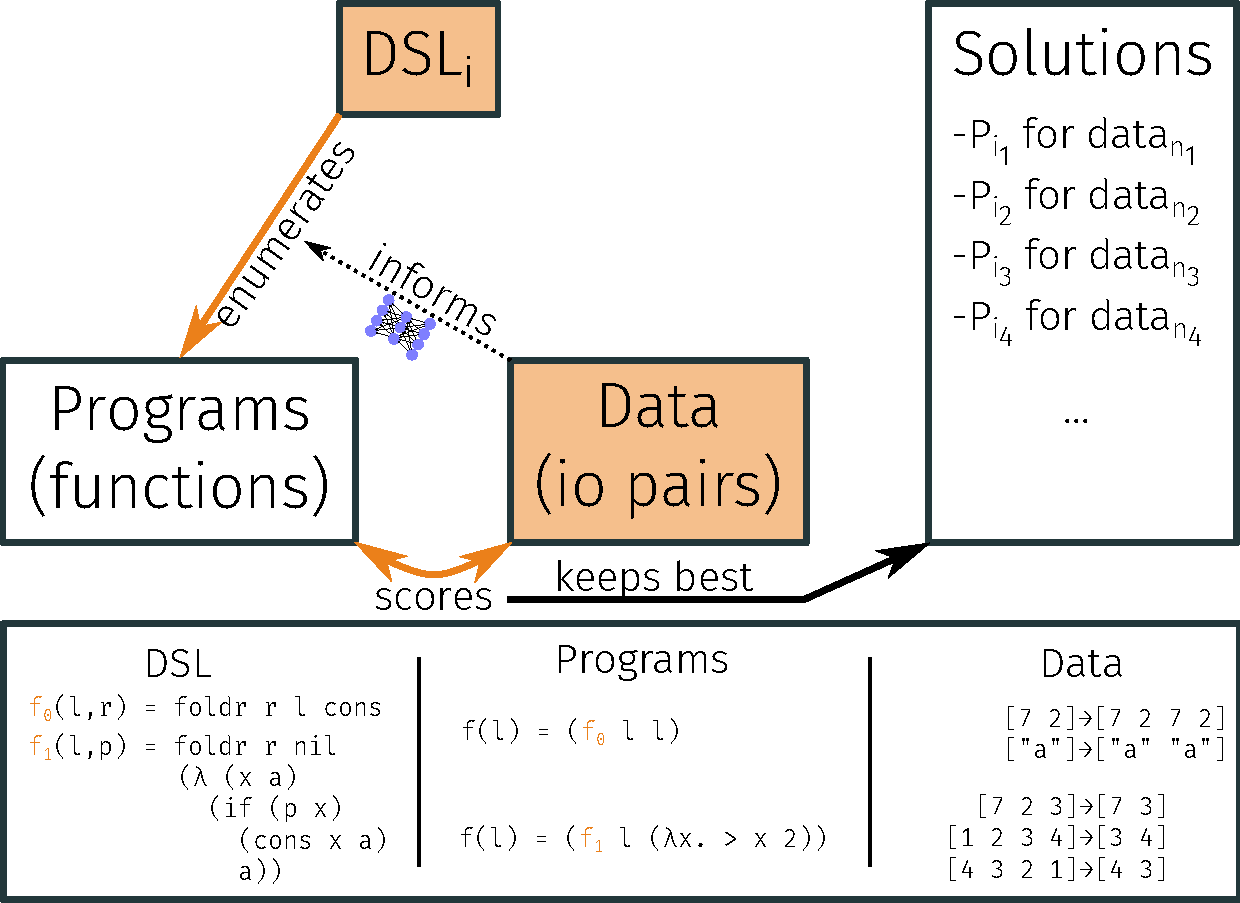
\includegraphics[width=11cm]{figures/teachDC/.inkslides-dc/slide-4.pdf}
  }

\end{frame}

\begin{frame}{DreamCoder --- Sleep-G}
  \only<1>{
    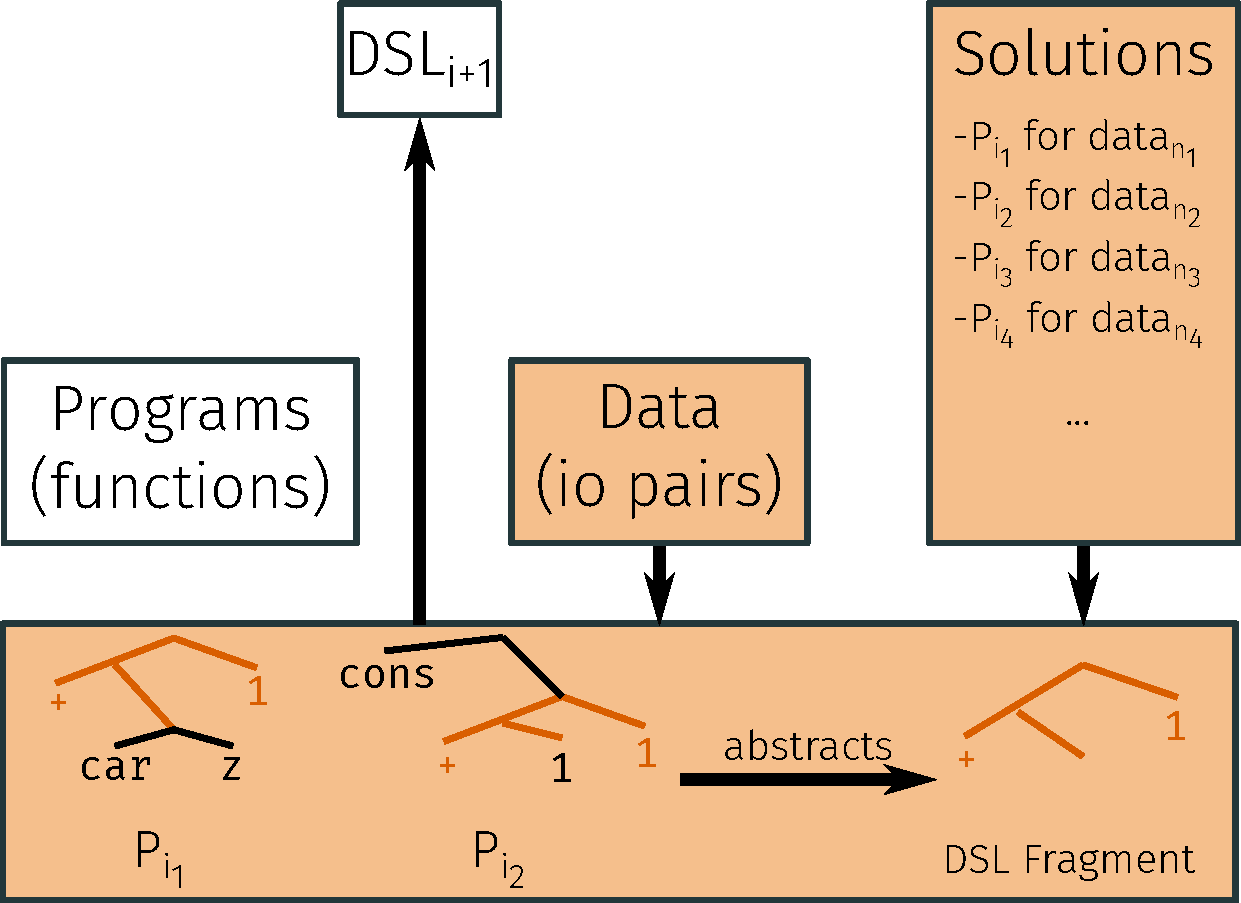
\includegraphics[width=11cm]{figures/teachDC/.inkslides-sleep-g/slide-4.pdf}
  }
\end{frame}


\begin{comment}

\begin{frame}{DreamCoder --- Sleep-G (\textbf{Refactoring})}
  \textbf{Learning higher-order \texttt{map} function}
  \Wider[5.4em]{
  \begin{tabular}{cc}
    \toprule Task&Program\\\midrule
    \begin{tabular}{l}
      \texttt{(1 2 3)}$\to$\texttt{(2 4 6)}\\
      \texttt{(1 9 2)}$\to$\texttt{(2 18 4)}\\
    \end{tabular}&

    \begin{tabular}{l}
      \texttt{(Y ($\lambda$ (r l) (if (nil? l) nil}\\
      \texttt{ (cons (+ (car l) (car l))}\\
      \phantom{\texttt{(cons }}\texttt{ (r (cdr l))))))}
    \end{tabular}\\\midrule
    \begin{tabular}{l}
      \texttt{(1 2 3)}$\to$\texttt{(2 3 4)}\\
      \texttt{(1 9 2)}$\to$\texttt{(2 10 3)}\\
    \end{tabular}&
    \begin{tabular}{l}
      \texttt{(Y ($\lambda$ (r l) (if (nil? l) nil}\\
      \texttt{ (cons (+ (car l) 1)}\\
      \phantom{\texttt{(cons }}\texttt{ (r (cdr l))))))}
    \end{tabular}
    
    \\\bottomrule
  \end{tabular}}

     \visible<2->{
      \centering
      \begin{tabular}{l}
          \texttt{\emph{map}} = \orange{\texttt{($\lambda$ (f) (Y ($\lambda$ (r l) (if (nil? l) nil}}\\
  \phantom{\texttt{\emph{map}} = \texttt{($\lambda$ (f) (Y ($\lambda$ (r l) (if }}\orange{\texttt{(cons (f (car l))}}\\
  \phantom{\texttt{\emph{map}} = \texttt{($\lambda$ (f) (Y ($\lambda$ (r l) (if }}\orange{\texttt{(r (cdr l))))))}}
      \end{tabular}
}
\end{frame}

\begin{frame}{DreamCoder --- Sleep-G (\textbf{Refactoring})}
  \textbf{Learning higher-order \texttt{map} function}
    \Wider[5.4em]{
  \begin{tabular}{cc}
    \toprule Task&Program\\\midrule
    \begin{tabular}{l}
      \texttt{(1 2 3)}$\to$\texttt{(2 4 6)}\\
      \texttt{(1 9 2)}$\to$\texttt{(2 18 4)}\\
    \end{tabular}&
\begin{tabular}{l}
\texttt{(}\orange{\texttt{($\lambda$ (f) (Y ($\lambda$ (r l) (if (nil? l) nil}}\\
\phantom{(($\lambda$ (f) (Y ($\lambda$ (r l)}\orange{\texttt{(cons (f (car l))}}\\
\phantom{(($\lambda$ (f) (Y ($\lambda$ (r l)}\orange{\texttt{(r (cdr l)))))))}}\\
\texttt{ ($\lambda$ (z) (+ z z)))}
      \end{tabular}

    \begin{tabular}{l}
    \end{tabular}\\\midrule
    \begin{tabular}{l}
      \texttt{(1 2 3)}$\to$\texttt{(2 3 4)}\\
      \texttt{(1 9 2)}$\to$\texttt{(2 10 3)}\\
    \end{tabular}
    &
    \begin{tabular}{l}
\begin{tabular}{l}
\texttt{(}\orange{\texttt{($\lambda$ (f) (Y ($\lambda$ (r l) (if (nil? l) nil}}\\
\phantom{(($\lambda$ (f) (Y ($\lambda$ (r l)}\orange{\texttt{(cons (f (car l))}}\\
\phantom{(($\lambda$ (f) (Y ($\lambda$ (r l)}\orange{\texttt{(r (cdr l)))))))}}\\
\texttt{ ($\lambda$ (z) (+ z 1)))}
      \end{tabular}
    \end{tabular}
    
    \\\bottomrule
  \end{tabular}}


      \centering
\begin{tabular}{l}
          \texttt{\emph{map}} = \orange{\texttt{($\lambda$ (f) (Y ($\lambda$ (r l) (if (nil? l) nil}}\\
  \phantom{\texttt{\emph{map}} = \texttt{($\lambda$ (f) (Y ($\lambda$ (r l) (if }}\orange{\texttt{(cons (f (car l))}}\\
  \phantom{\texttt{\emph{map}} = \texttt{($\lambda$ (f) (Y ($\lambda$ (r l) (if }}\orange{\texttt{(r (cdr l))))))}}
      \end{tabular}

\end{frame}

\begin{frame}[plain]{}\footnotesize
  \Wider[5.4em]{
    \begin{tikzpicture}[every node/.style={inner sep=0,outer sep=0}]
    \node(p1)[draw] at (-1,0) {
      \begin{tabular}{l}
      \texttt{(Y ($\lambda$ (r l) (if (nil? l) nil}\\
      \texttt{ (cons (+ (car l) (car l))}\\
      \phantom{\texttt{(cons }}\texttt{ (r (cdr l))))))}
    \end{tabular}
    };
    \node(r1)[draw,inner sep=0,outer sep=0] at ([yshift=-3cm]p1.south) {
      \begin{tabular}{l}
  \texttt{(}\orange{\texttt{($\lambda$ (f) (Y ($\lambda$ (r l) (if (nil? l)}}\\
\phantom{(($\lambda$ (f) (Y ($\lambda$ (r l)}\orange{\texttt{nil}}\\
\phantom{(($\lambda$ (f) (Y ($\lambda$ (r l)}\orange{\texttt{(cons (f (car l))}}\\
\phantom{(($\lambda$ (f) (Y ($\lambda$ (r l)}\orange{\texttt{ (r (cdr l)))))))}}\\
\texttt{ ($\lambda$ (z) (+ z z)))}
      \end{tabular}
    };

        \node(p2)[draw] at ([xshift=3.5cm]p1.east) {
    \begin{tabular}{l}
      \texttt{(Y ($\lambda$ (r l) (if (nil? l) nil}\\
      \texttt{ (cons (+ (car l) 1)}\\
      \phantom{\texttt{(cons }}\texttt{ (r (cdr l))))))}
    \end{tabular}
    
    };
    \node(r2)[draw] at ([yshift=-3cm]p2.south) {
\begin{tabular}{l}
  \texttt{(}\orange{\texttt{($\lambda$ (f) (Y ($\lambda$ (r l) (if (nil? l)}}\\
\phantom{(($\lambda$ (f) (Y ($\lambda$ (r l)}\orange{\texttt{nil}}\\
\phantom{(($\lambda$ (f) (Y ($\lambda$ (r l)}\orange{\texttt{(cons (f (car l))}}\\
\phantom{(($\lambda$ (f) (Y ($\lambda$ (r l)}\orange{\texttt{ (r (cdr l)))))))}}\\
\texttt{ ($\lambda$ (z) (+ z 1)))}
      \end{tabular}

    };

    \draw [->] (p1.south)  --(r1.north) node[fill=white,midway] {refactor};
    \draw [->] (p2.south)  --(r2.north) node[fill=white,midway] {refactor};

    \node[draw](m) at (2,-7) {
\begin{tabular}{l}
          \texttt{\emph{map}} = \orange{\texttt{($\lambda$ (f) (Y ($\lambda$ (r l) (if (nil? l) nil}}\\
  \phantom{\texttt{\emph{map}} = \texttt{($\lambda$ (f) (Y ($\lambda$ (r l) (if }}\orange{\texttt{(cons (f (car l))}}\\
  \phantom{\texttt{\emph{map}} = \texttt{($\lambda$ (f) (Y ($\lambda$ (r l) (if }}\orange{\texttt{(r (cdr l))))))}}
      \end{tabular}      
    };
    \draw [->](r1.south)--(m.north);
    \draw [->](r2.south)--(m.north);
    \node[fill=white] at ([yshift=0.5cm]m.north) {\textbf{Compress (MDL/Bayes objective)}};
    \visible<2-3>{
      \node[fill=orange!50!white,align=center] at (r1) {\Huge $10^{14}$\\\Huge  refactorings };
      \node[fill=orange!50!white,align=center] at (r2) {\Huge $10^{13}$\\\Huge  refactorings };
    }
    \visible<3>{
      \node[fill=orange!50!white,align=center] at ([yshift=7cm]m.north) {\Huge version space: set of programs\\
      \huge Lau 2003; Gulwani 2012};
      }
    \visible<4>{
      \node[fill=orange!50!white,align=center] at (r1) {\Huge $\leq 10^6$\\\Huge version spaces };
      \node[fill=orange!50!white,align=center] at (r2) {\Huge $\leq 10^6$\\\Huge version spaces };
    }
    \end{tikzpicture}
    }
\end{frame}
 \end{comment}




\begin{frame}{DreamCoder --- Sleep-R (\textbf{Experience Replay})}
  \only<1>{
    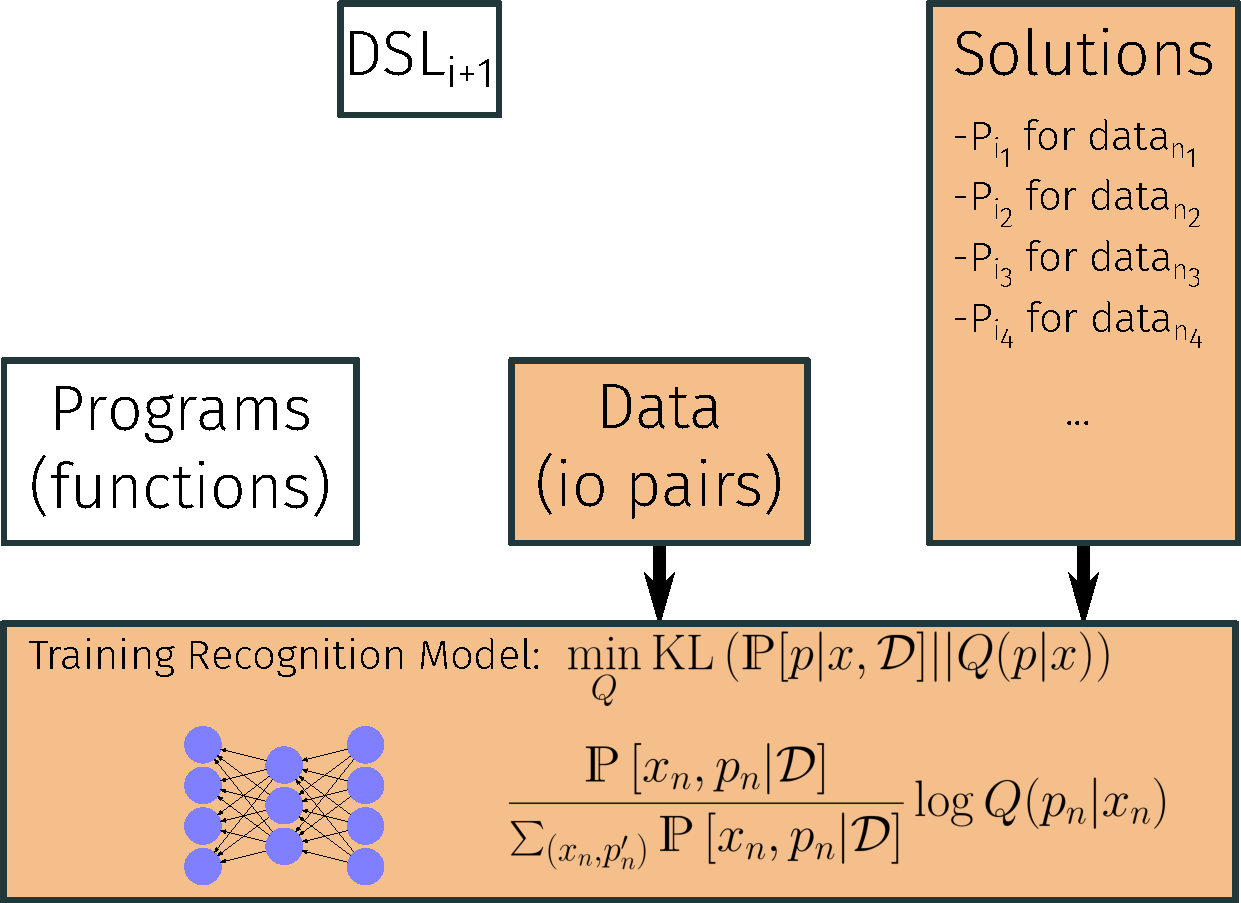
\includegraphics[width=11cm]{figures/teachDC/.inkslides-sleep-r-1/slide-4.pdf}
  }
\end{frame}
\begin{frame}{DreamCoder --- Sleep-R (\textbf{Dreaming})}
  \only<1>{
    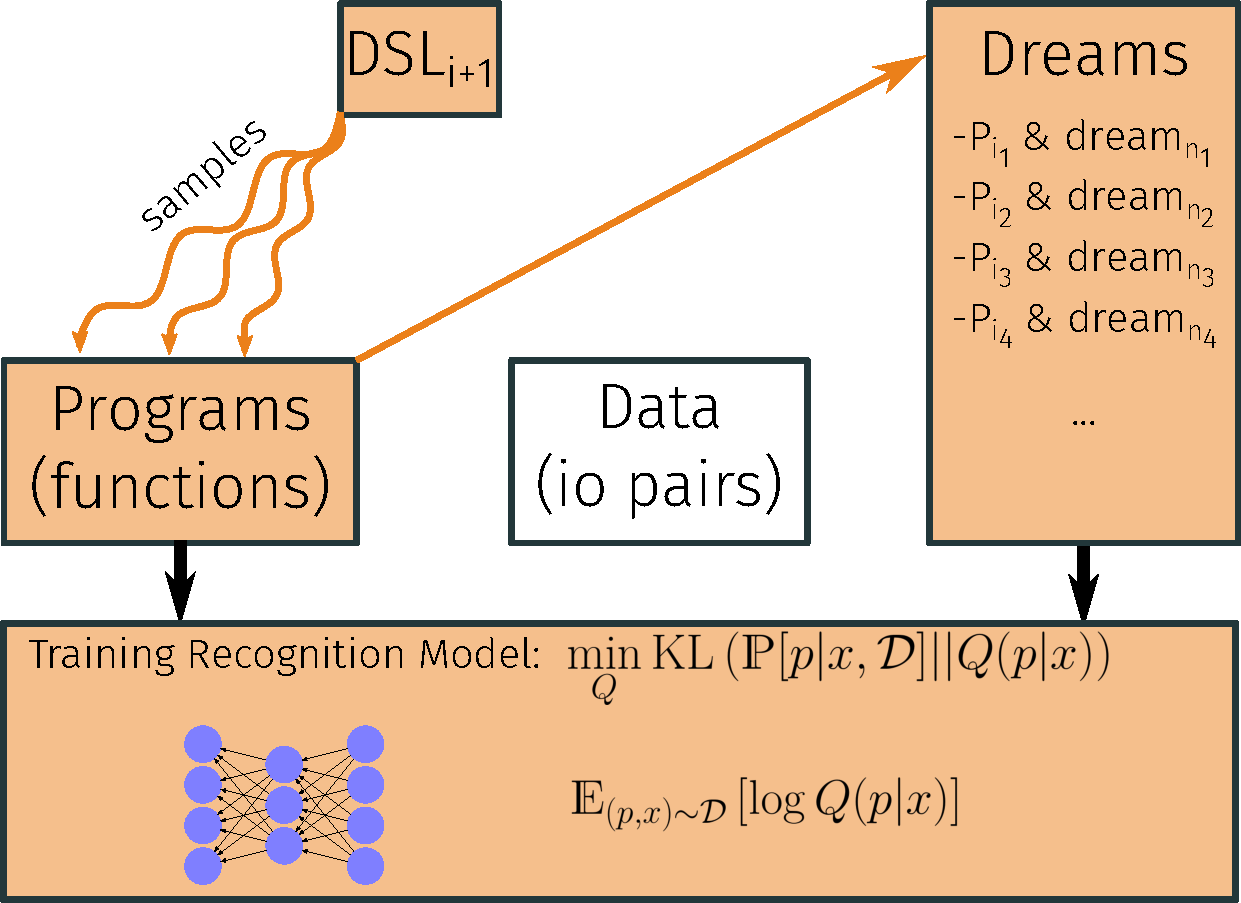
\includegraphics[width=11cm]{figures/teachDC/.inkslides-sleep-r-2/slide-4.pdf}
  }
\end{frame}
 

\begin{frame}{List functions --- \small{Created \& investigated by Lucas
  Morales}}


  \vspace{1cm}
  
  \begin{figure}[b]\centering
\vspace{-0.5cm}  \begin{tabular}{lll}
    \toprule
    Name & Input & Output \\\midrule
    repeat-3 & [7\, 0] & [7\, 0\, 7\, 0\, 7\, 0] \\
    drop-3 & [0\, 3\, 8\, 6\, 4] & [6\, 4] \\
    rotate-2 & [8\, 14\, 1\, 9] & [1\, 9\, 8\, 14] \\
    count-head-in-tail & [1\, 2\, 1\, 1\, 3] & 2 \\
    keep-div-5 & [5\, 9\, 14\, 6\, 3\, 0] & [5\, 0] \\
    product & [7\, 1\, 6\, 2] & 84 \\
    \bottomrule
  \end{tabular}
  %\captionof{table}{Some tasks in our list function domain.}\label{listExamples}\vspace{-0.5cm}
\end{figure}

  Discovers 38 concepts, including `filter'. %With different tasks will also learn `map', `fold', `unfold', etc. starting with 1950's Lispthe
  
\begin{picture}(50,70) \put(250,0){\hbox{\includegraphics[width = 3cm]{figures/Lucas}}} \end{picture} 
\end{frame}


\begin{frame}{Text editing}
  In the style of FlashFill (Gulwani 2012)

  \centering  \includegraphics[width = 5cm]{textColumn.png}

\vspace{-0.5cm}  SyGuS problems: solves 3\% before learning, vs 75\% after learning. Best prior work: 80\%

\end{frame}

\begin{frame}{List functions \& Text editing: Learning curves on hold out tasks}

  \begin{center}
    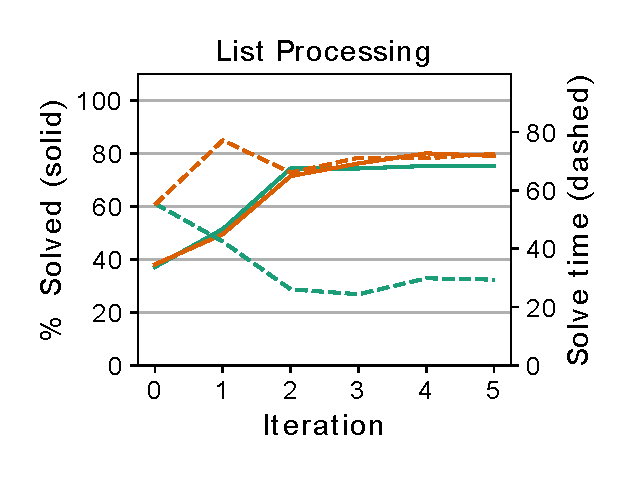
\includegraphics[width = 5cm]{figures/listLearningCurve.eps}
\hfill    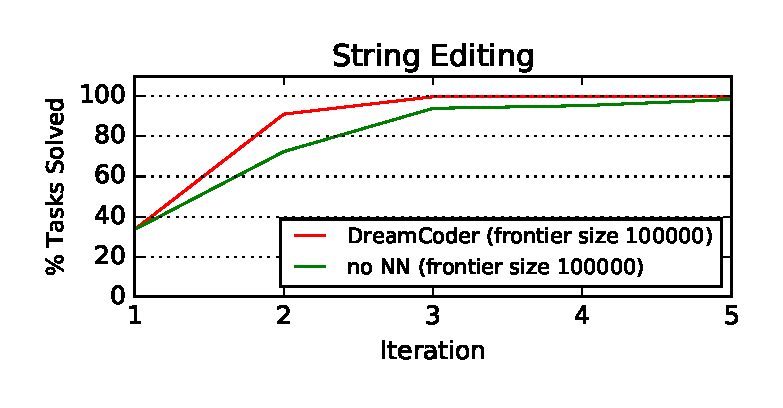
\includegraphics[width = 5cm]{figures/textLearningCurve.eps} 
    \end{center}

Learning curves for DreamCoder both with (\orange{in orange}) and without
    (\teal{in teal}) the recognition model. Solid lines: \% holdout testing tasks solved w/ 10m timeout. Dashed lines: Average solve time, averaged only over tasks that are solved.


\end{frame}


\begin{frame}{Learned text processing DSL}
  \only<1>{  \includegraphics[width = \textwidth]{figures/textPrimitives.pdf}}
  \only<2>{  \includegraphics[width = \textwidth]{figures/textPrimitives.png}}

\end{frame}

\begin{frame}{Learning the fundamentals of programming}
  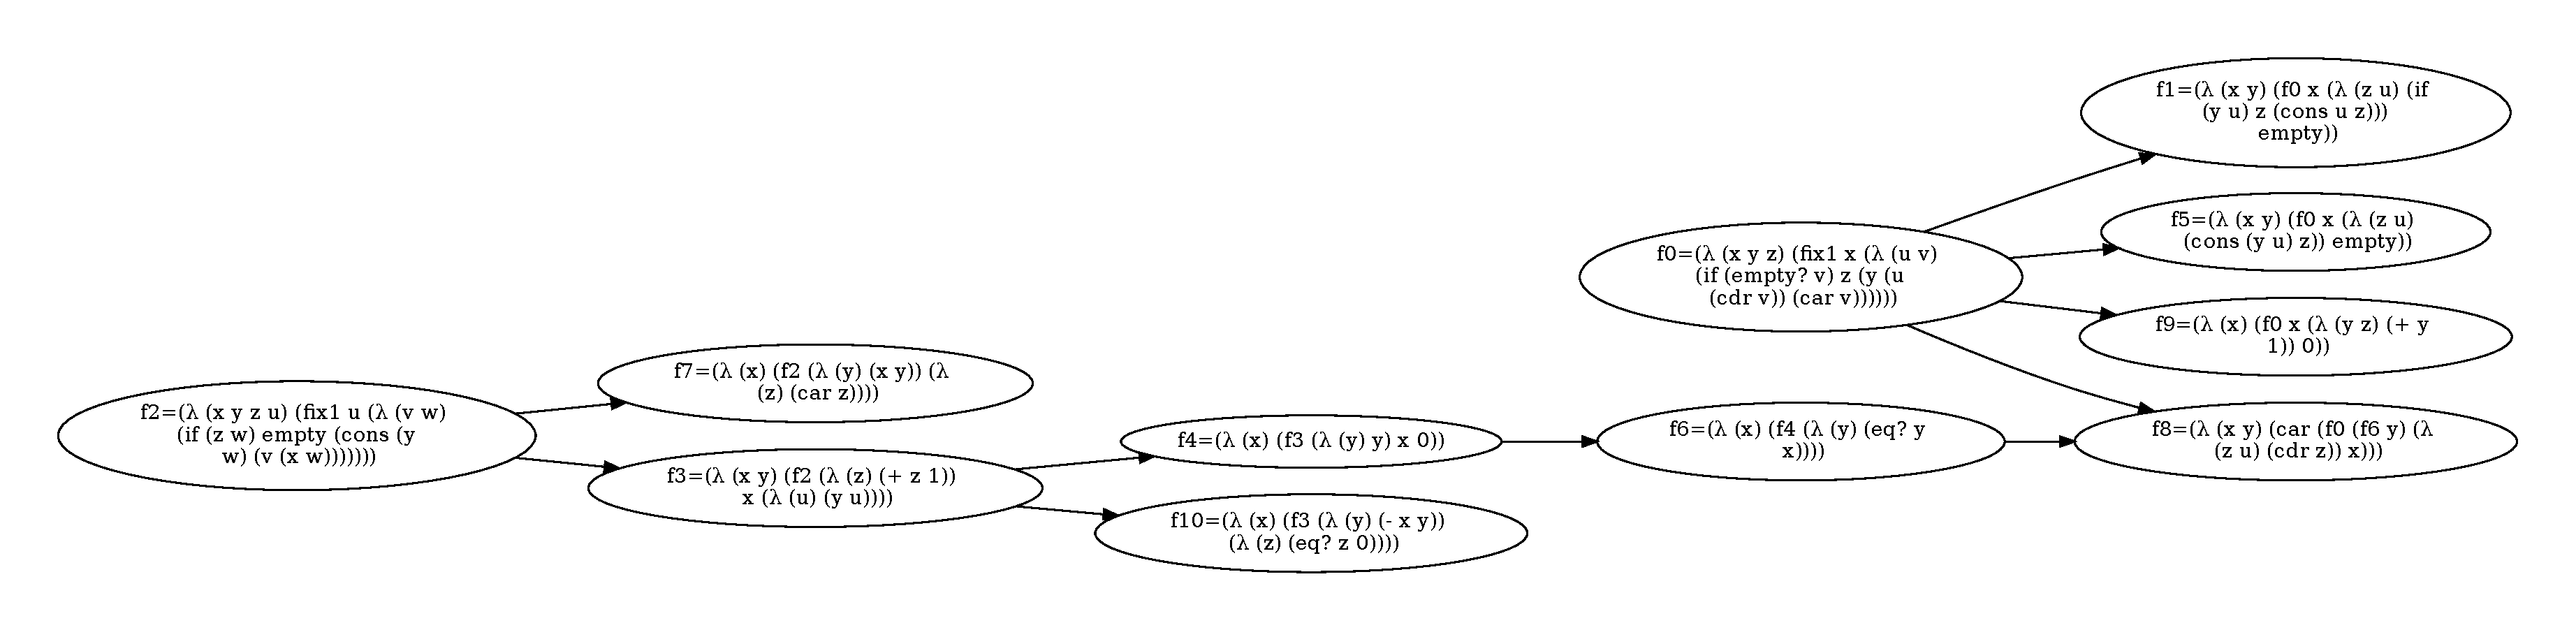
\includegraphics[width = \textwidth]{figures/McCarthy.png}

\centering  McCarthy 1959 Lisp  $\longrightarrow$ Modern functional programming
  
  22 tasks. 64 CPUs. 93 hours.

  \end{frame}

\begin{frame}{Symbolic regression from visual input}
\centering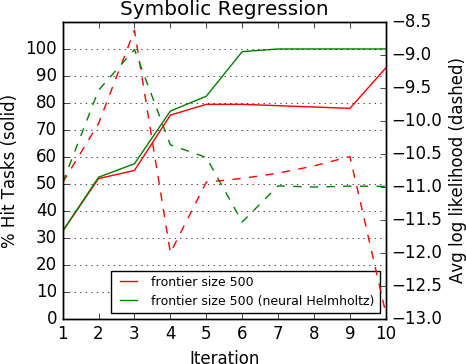
\includegraphics[width = 5cm]{symbolicRegression.png}
\end{frame}

\begin{frame}{Turtle graphics --- \small{Created \& investigated by Mathias
      Sablé--Meyer}}
    \begin{picture}(50,50) \put(280,-20){\hbox{\includegraphics[width = 2cm]{figures/French}}} \end{picture} \vspace{-2cm}

  \begin{block}{DSL}
    \texttt{OP ::= FW x | RT x | UP | DOWN | SET state}
  \end{block}

  \begin{block}{Tasks}
    \texttt{task : image}
  \end{block}

  \vspace{0.2cm}

  \only<1>{
    \begin{columns}[T]
      \column{0.5 \textwidth}
        \begin{mycode}
          \texttt{FW 1}\\
          \vspace*{5\baselineskip}
        \end{mycode}
      \column{0.5 \textwidth}
        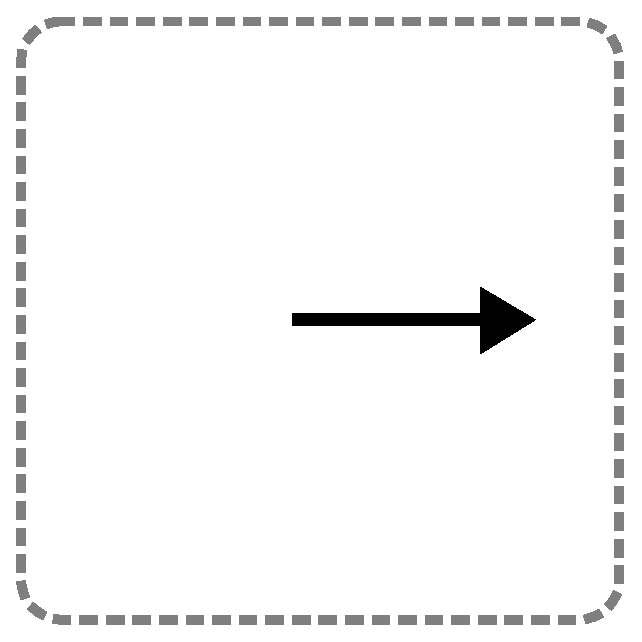
\includegraphics[width = 4cm]{figures/teachLogo/line.eps}
    \end{columns}
  }
  \only<2>{
    \begin{columns}[T]
      \column{0.5 \textwidth}
        \begin{mycode}
          \texttt{FW 1}\\
          \texttt{RT} $\frac\pi2$\\
          \texttt{FW 1}\\
          \vspace*{3\baselineskip}
        \end{mycode}
      \column{0.5 \textwidth}
        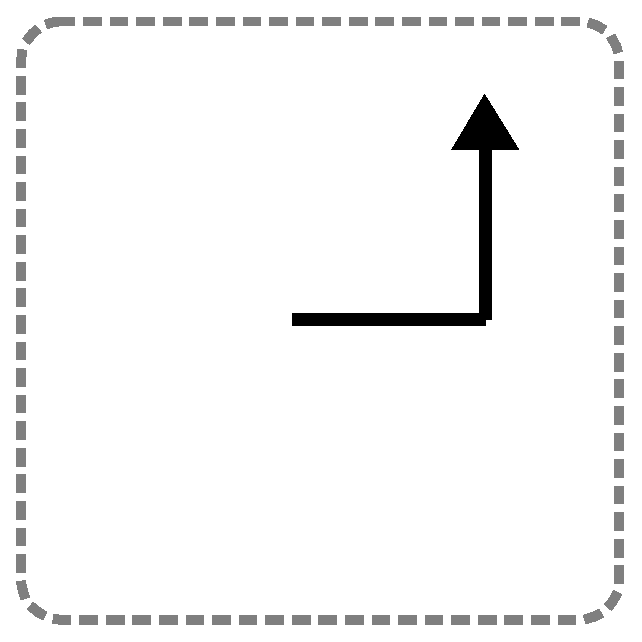
\includegraphics[width = 4cm]{figures/teachLogo/angle.eps}
    \end{columns}
  }
  \only<3>{
    \begin{columns}[T]
      \column{0.5 \textwidth}
        \begin{mycode}
          \texttt{FW 1}\\
          \texttt{RT} $\frac\pi2$\\
          \texttt{FW 1}\\
          \texttt{RT} $\frac\pi2$\\
          \texttt{FW 1}\\
          \vspace*{1\baselineskip}
        \end{mycode}
      \column{0.5 \textwidth}
        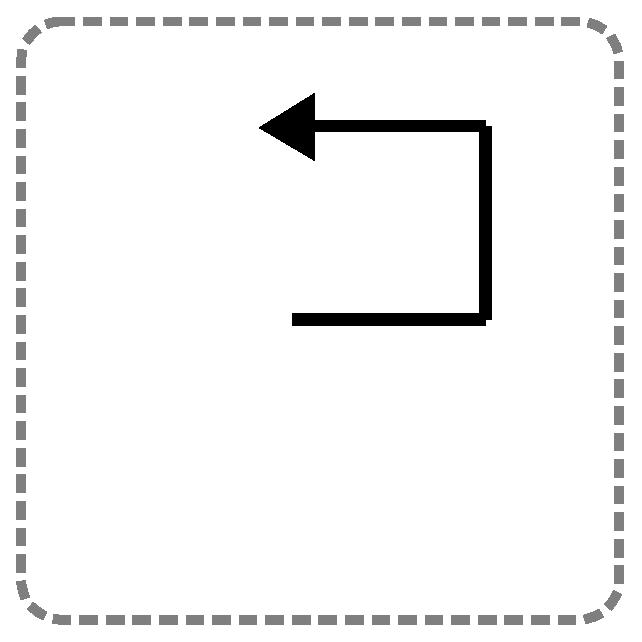
\includegraphics[width = 4cm]{figures/teachLogo/angle2.eps}
    \end{columns}
  }
  \only<4>{
    \begin{columns}[T]
      \column{0.5 \textwidth}
        \begin{mycode}
          \texttt{for i in range(4)}\\
          \texttt{> FW 1}\\
          \texttt{> RT} $\frac\pi2$\\
          \vspace*{3\baselineskip}
        \end{mycode}
      \column{0.5 \textwidth}
        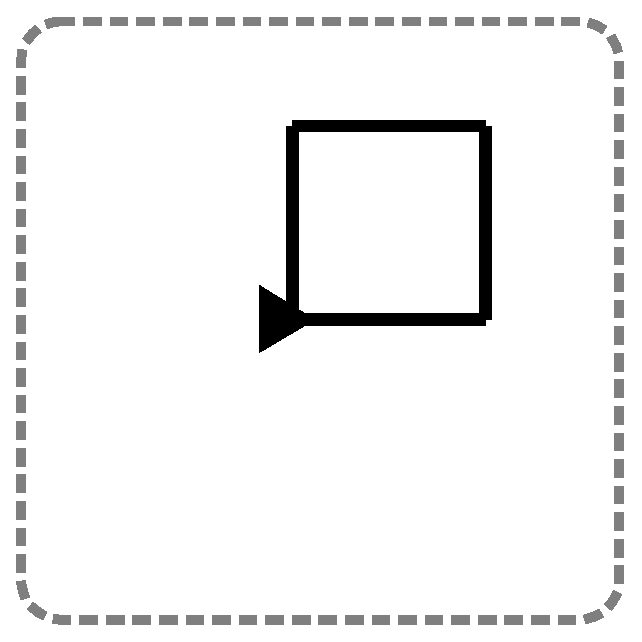
\includegraphics[width = 4cm]{figures/teachLogo/square.eps}
    \end{columns}
  }
  \only<5>{
    \begin{columns}[T]
      \column{0.5 \textwidth}
        \begin{mycode}
          \texttt{for i in range(8)}\\
          \texttt{> FW 1} \\
          \texttt{> SET origin} \\
          \texttt{> RT} $\frac{2\pi}{8}$\\
          \vspace*{2\baselineskip}
        \end{mycode}
      \column{0.5 \textwidth}
        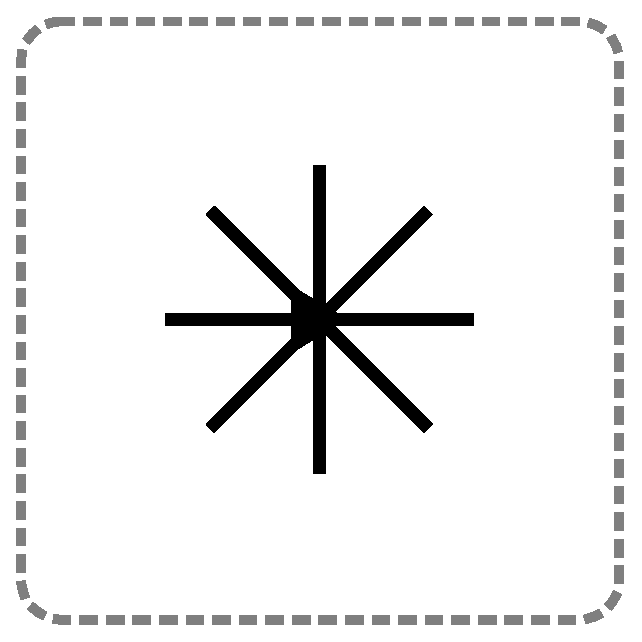
\includegraphics[width = 4cm]{figures/teachLogo/star.eps}
    \end{columns}
  }
  \only<6>{
    \begin{columns}[T]
      \column{0.5 \textwidth}
        \begin{mycode}
          \texttt{for i in range(8)}\\
          \texttt{> PU} \\
          \texttt{> FW} $\frac{\text{\texttt{i}}}{2}$\\
          \texttt{> PD} \\
          \texttt{> FW} $\frac{\text{\texttt{i}}}{2}$\\
          \texttt{> RT} $\frac\pi2$\\
          \vspace*{0\baselineskip}
        \end{mycode}
      \column{0.5 \textwidth}
        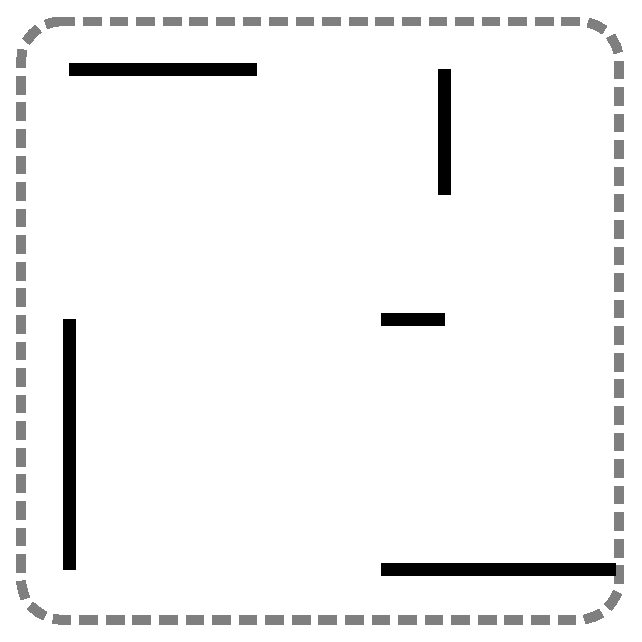
\includegraphics[width = 4cm]{figures/teachLogo/spiral.eps}
    \end{columns}
  }
  \only<7>{
    \begin{columns}[T]
      \column{0.5 \textwidth}
        \begin{mycode}
          \texttt{for i in range($\infty$)}\\
          \texttt{> FW $\varepsilon$}\\
          \texttt{> RT} $\varepsilon$\\
          \vspace*{3\baselineskip}
        \end{mycode}
      \column{0.5 \textwidth}
        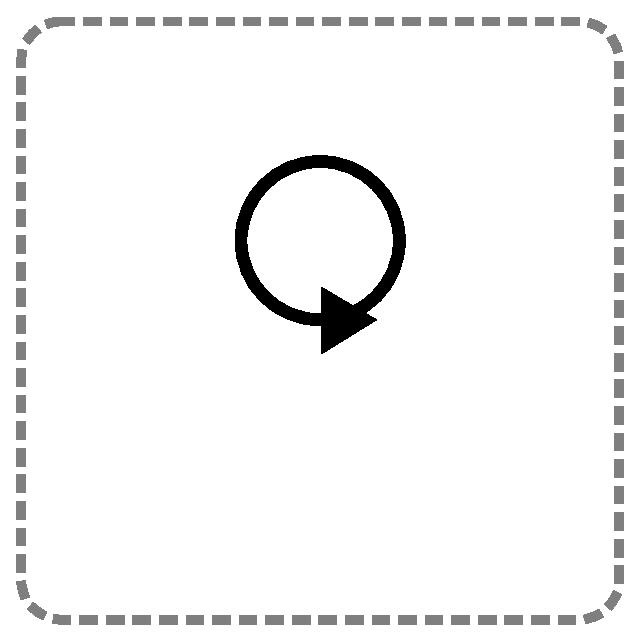
\includegraphics[width = 4cm]{figures/teachLogo/circle.eps}
    \end{columns}
  }
  \visible<7>{
    \vspace{0.2cm}
    \texttt{\alert{NUM} ::= 1 | $\pi$ | $\infty$ | $\varepsilon$ | + | - | * | / }
  }

\end{frame}

\begin{frame}{Turtle graphics --- Training tasks}
  \centering
  \includegraphics[width=11cm]{figures/tasksMinusBehaviour.png}
\end{frame}

%% \begin{frame}{Turtle graphics --- Learning curves}
%%   \centering
%%   \includegraphics[width=9cm]{figures/dreams/montageTalkLC.eps}
%%   %% \begin{itemize}
%%   %%   \item $\frac\pi2$ and $\frac\pi4$ from $\pi$, $2$, $+$ and $/$
%%   %%   \item A line of length \texttt{n} followed with a right angle
%%   %%   \item Loops of length \texttt{n} that uses the number \texttt{n} inside.
%%   %%   \item Unit line then teleport back to origin
%%   %%   \item ...
%%   %% \end{itemize}
%% \end{frame}

\begin{frame}{Turtle graphics --- Illustration of learned DSL}

  \only<1>{\centering\includegraphics[width = 0.3\textwidth]{figures/logo_primitives/logo_primitive_4.png}}
  \only<2>{\includegraphics[width = \textwidth]{figures/logo_primitives/logo_primitive_1.png}}
  \only<3>{\includegraphics[width = \textwidth]{figures/logo_primitives/logo_primitive_7.png}}
  \only<4>{\centering\includegraphics[width = \textwidth]{figures/logo_primitives/logo_primitive_12.png}}
  \only<5>{\centering\includegraphics[width = \textwidth]{figures/logo_primitives/logo_primitive_14.png}}
  \only<6>{\centering\includegraphics[width = \textwidth]{figures/logo_primitives/logo_primitive_5.png}}
%  \only<7>{\centering\includegraphics[width = \textwidth]{figures/logo_primitives/logo_primitive_13.png}}

  \end{frame}

\begin{frame}{Turtle graphics --- Dreams}
  \centering
  \includegraphics[width=7cm]{figures/dreams/montageTalkDreams.eps}
\end{frame}

%% \begin{frame}{Turtle graphics --- More dreams, 5 minutes, 1st iteration}
%%   \centering
%%   \includegraphics[width=8cm]{figures/dreams/5m_firstIteration.eps}
%% \end{frame}

%% \begin{frame}{Turtle graphics --- More dreams, 5 minutes, last iteration}
%%   \centering
%%   \includegraphics[width=8cm]{figures/dreams/5m_final.eps}
%% \end{frame}

\begin{frame}{Turtle graphics --- Dreaming from learned generative model}
  \centering
  \only<1>{
    \begin{figure}
      \includegraphics[width=6cm]{figures/dreams/1.png}
    \end{figure}
  }
  \only<2>{
    \begin{figure}
      \includegraphics[width=6cm]{figures/dreams/2.png}
    \end{figure}
  }
  \only<3>{
    \begin{figure}
      \includegraphics[width=6cm]{figures/dreams/3.png}
    \end{figure}
  }
  \only<4>{
    \begin{figure}
      \includegraphics[width=6cm]{figures/dreams/4.png}
    \end{figure}
  }
  \only<5>{
    \begin{figure}
      \includegraphics[width=6cm]{figures/dreams/6.png}
    \end{figure}
  }
  \only<6>{
    \begin{figure}
      \includegraphics[width=6cm]{figures/dreams/7.png}
    \end{figure}
  }
  \only<7>{
    \begin{figure}
      \includegraphics[width=6cm]{figures/dreams/8.png}
    \end{figure}
  }
  \only<8>{
    \begin{figure}
      \includegraphics[width=6cm]{figures/dreams/9.png}
    \end{figure}
  }
\end{frame}

\begin{comment}
\begin{frame}{Tower building in blocks world}
  \large
\centering  
  Control a hand that puts down blocks \\
  \hspace{1cm}(turtle: control a pen that puts down ink)
\only<1>{\includegraphics[width = \textwidth]{figures/3t.png}}
\only<2>{\includegraphics[width = 0.6\textwidth]{figures/every_tower.png}}
  

  \end{frame}

\begin{frame}{Tower building in blocks world: Learned concepts}
  Parametric planning primitives. Example pyramid concept:

  \includegraphics[width = \textwidth]{figures/pyramid.png}

\end{frame}

\begin{frame}{Tower building in blocks world: Learned concepts}
  Parametric planning primitives. Example brickwall concept:

  \includegraphics[width = \textwidth]{figures/brickwall.png} 

\end{frame}
  \end{comment}

\begin{frame}{Vision}


   \underline{More human-like machine intelligence}\\%Flexibly adapting to new problem domains:
   \begin{itemize}
   \item    Acquiring a domain-specific representation (DSL)
     \item Learning  to use that representation (recognition model)
   \end{itemize}
   DreamCoder: an algorithm for jointly realizing these goals

   



   \hspace{-1cm}\includegraphics[width = 12cm]{figures/finale.png}

   \pause

   \Huge \centering \textbf{The End.}
  \end{frame}

\end{document}
